\documentclass[12pt,prb,aps]{revtex4-1}
\usepackage {amsmath}
\usepackage{amssymb}
%\pdfoutput = 1 
\usepackage {graphicx}
\newcommand{\bomega}{\mbox{\boldmath$\omega$}}
\allowdisplaybreaks

\begin{document}

\title{Theoretical Investigation of the Triggering of Neoclassical Tearing Modes by Transient Resonant Magnetic Perturbations in NSTX}
\author{R.~Fitzpatrick\,\footnote{rfitzp@utexas.edu}}
\affiliation{Institute for Fusion Studies,  Department of Physics,  University of Texas at Austin,  Austin TX 78712, USA.}

\begin{abstract}

\end{abstract}

\maketitle

\section{Introduction}
Neoclassical tearing modes (NTMs) are the main obstacle to obtaining
normalized plasma pressure ($\beta$) levels in tokamak\,\cite{wesson} plasmas that are adequate for  achieving 
thermonuclear fusion.\cite{buttery,lahaye} NTMs were originally identified experimentally on the TFTR tokamak.\cite{tftr} NTMs lead to the generation of low poloidal and toroidal mode number ($m$ and $n$) magnetic island chains on toroidal magnetic flux-surfaces within the plasma that are characterized by rational (i.e., $m/n$) values of the safety-factor ($q$). An NTM is driven by a helical hole in the bootstrap current\,\cite{boot} profile  that arises as a consequence of the flattening of the
plasma pressure across the associated island chain region.\cite{carrera} However, a magnetic island chain can only locally flatten
the plasma pressure  when its radial width exceeds a certain threshold value that depends on the local ratio of the
parallel and perpendicular energy diffusivities.\cite{fitz} This  leads to the conclusion that NTMs are actually meta-stable.
In other words, some sort of seed perturbation must be applied to the relevant rational magnetic flux-surface in order to trigger an NTM. In practice, the seed perturbation usually takes the form of a transient magnetic perturbation that is resonant at the
rational surface. Such perturbations are generated in tokamak plasmas primarily by sawtooth crashes, edge localized modes, and fishbones.\cite{buttery,lahaye} 

The aim of this paper is to investigate how the properties (i.e., amplitude, duration, and rotation frequency) of a transient resonant
magnetic perturbation (RMP) applied to a toroidal tokamak plasma affect its ability to trigger NTMs within the plasma. In this
study, we shall use the EPEC code (see Sect.~\ref{epecc}) to simulate what happens when a transient  $n=1$  magnetic
perturbation  is applied to a typical NSTX plasma. 

\section{Brief Description of EPEC Code}\label{epecc}
The EPEC code\,\cite{rftor,rftor1,rftor2,rftor3} employs an asymptotic matching\,\cite{fkr,coppi,ruth,ara,tt1,tt2,tt3,tt4,tt5,tt6,tt7} approach to determine the resistive response of a toroidal tokamak equilibrium to an applied RMP.
The main advantage of the asymptotic matching approach is that it largely removes the very short Alfv\'{e}n time from the problem. In fact, the EPEC
code is capable of accurately simulating the resistive response of a toroidal tokamak plasma to an RMP while taking time steps that extend over many Alfv\'{e}n times. 
In this manner, the code is able to simulate a complete plasma discharge in a matter of minutes of real time. 

The version of the EPEC model used in this paper is described in detail in Appendix~\ref{epec}. 
The EPEC model is fully toroidal, and makes use of experimental magnetic equilibrium data (gfiles)  and plasma profile data (pfiles). The model incorporates an accurate neoclassical model\,\cite{sigmar} that takes impurities and neutral particles into account, and  allows the calculation of the neoclassical poloidal flow-damping timescale, the 
charge-exchange damping timescale, the neoclassical ion rotation profile, and the bootstrap current profile. The model also includes  perturbed bootstrap current, magnetic field-line curvature, ion polarization current, and island saturation terms in the resonant plasma response model that governs the growth of magnetic island chains at the various rational surfaces within the plasma. Finally, the model accurately calculates the critical
island widths needed to locally flatten the plasma pressure profile. 

\section{NSTX Discharge 127317}
\subsection{Introduction}
The two NSTX discharges studied in this paper were chosen because they were both fairly generic and had precomputed  kinetic-EFITs. 

The first discharge studied in this paper is 127317, which was one of the discharges used in an investigation of the interaction between
edge localized modes (ELMs) and RMPs in NSTX.\cite{nstx} Discharge 127317 is an H-mode discharge, characterized by a double magnetic null boundary shape,  6 MW of neutral
beam heating power, and no lithium coating of the walls. 

\subsection{Magnetic Equilibrium}
Figure~\ref{fig1} shows the magnetic equilibrium of NSTX discharge 127317 at $t=400$ ms. This equilibrium is characterized by a scale major radius
$R_0=0.85$ m (see Sect.~\ref{a1}), a scale toroidal magnetic field-strength $B_0=0.44$ T (see Sect.~\ref{a2}), a net toroidal plasma current $I_\phi = 753$ kA, a safety-factor at the 95\% flux-surface $q_{95} = 11.0$, and a poloidal beta $\beta_p=0.61$. 

\subsection{Plasma Profiles}
Figure~\ref{fig2} shows the safety-factor, electron number density, electron temperature, impurity ion number density, and impurity ion toroidal angular velocity profiles in NSTX discharge 127317 at $t=400$ ms. The majority ions are deuterium, and the impurities are assumed to
be fully-stripped carbon ions. Note that the discharge is subject to rotation braking due to an applied $n=3$ RMP, which accounts for the lower than usual toroidal rotation. Because there is no
poloidal impurity ion rotation data for this discharge, the ${\bf E}\times {\bf B}$ rotation profile is deduced from the
toroidal  impurity ion rotation data using neoclassical theory. (See Sect.~\ref{srotation}.) 

The perpendicular electron energy diffusivity ($\chi_e$), perpendicular ion energy diffusivity ($\chi_i$), perpendicular toroidal momentum diffusivity ($\chi_\phi$), and perpendicular particle diffusivity ($D_\perp$) are given the plausible values $1.0$, $1.0$, $1.0$, and $0.2$
${\rm m}^2/{\rm s}$, respectively,  throughout the plasma.

 The flux-surface averaged neutral deuterium atom number density takes the form $\langle n_n\rangle(r) = \langle n_n\rangle(r_{100})/[1+(r-r_{100})^2/l_n^{\,2}]$, where
$\langle n_n\rangle(r_{100})= 1\times 10^{16}\,{\rm m}^{-3}$, and $l_n=1.3\times 10^{-2}\,{\rm m}$. The flux-surface neutral poloidal asymmetry parameter is given the value $y_n=1.5$. (See Sect.~\ref{sbalance}.) The flux-surface averaged deuterium-atom/deuterium-ion charge-exchange rate constant is $\langle \sigma\,v\rangle_i^{{\rm cx}} = 4\times 10^{-14}\,{\rm m}^{3}\,{\rm s}^{-1}$.\cite{barnett} The neutrals are assumed to be hot (i.e., $E_n/T_i=1$.) 
Note that neutrals do not really play a role in the physics of NTMs, which are resonant in the plasma core. 

\subsection{NTM Stability}

\section{NSTX Discharge 139057}
\subsection{Introduction}
The second discharge  studied in this paper is 139057, which was one of the discharges used in an investigation of blob dynamics in NSTX.\cite{nstx1} Discharge 139057 is an H-mode discharge, characterized by a single magnetic null boundary shape,  6 MW of neutral
beam heating power, and  lithium coating of the walls. 

\subsection{Magnetic Equilibrium}
Figure~\ref{fig11} shows the magnetic equilibrium of NSTX discharge 139057 at $t=557$ ms. This equilibrium is characterized by a scale major radius
$R_0=0.85$ m, a scale toroidal magnetic field-strength $B_0=0.54$ T, a net toroidal plasma current $I_\phi = 907$ kA, a safety-factor at the 95\% flux-surface $q_{95} = 9.5$, and a poloidal beta $\beta_p=0.57$. 

\subsection{Plasma Profiles}
Figure~\ref{fig12} shows the safety-factor, electron number density, electron temperature, impurity ion number density, and impurity ion toroidal angular velocity profiles in NSTX discharge 139057 at $t=557$ ms. As before, the majority ions are deuterium, and the impurities are assumed to
be fully-stripped carbon ions. Note that the discharge is not subject to rotation braking due to an applied $n=3$ RMP, which accounts for the higher toroidal rotation than that in discharge 127317. As before, the ${\bf E}\times {\bf B}$ rotation profile is deduced from the
toroidal  impurity ion rotation data using neoclassical theory. 

The diffusivity and neutral profiles in discharge 139057 are assumed to be the same as those adopted in the study of
discharge 127317. 

\subsection{NTM Stability}

\section{Summary and Conclusions}

\section*{Acknowledgements}
The author would also
like to thank J.-K.~Park and N.C.~Logan for their advice on how to run the GPEC code. Part of the data analysis was performed using
the OMFIT integrated modeling framework.\cite{omfit}

This research was directly funded by the U.S.\ Department of Energy, Office of Science, Office of Fusion Energy Sciences, under  contract DE-SC0021156. 

\appendix
\section{Description of EPEC Model}\label{epec}
\subsection{Introduction}
The (Extended Perturbed Equilibrium Code) EPEC model was introduced in Ref.~\onlinecite{rftor}, and imporved  in Refs.~\onlinecite{rftor1}, \onlinecite{rftor2}, and \onlinecite{rftor3}. The model has been further extended for the study
presented in this paper. 
The latest improvements to the model include the introduction of  perturbed bootstrap current, magnetic field-line
curvature, ion polarization current, and island saturation terms into the resonant plasma response model (see Sects.~\ref{ggjs}, \ref{sbalance}, \ref{sneo}, and \ref{res}), a more accurate calculation of the critical island widths needed to
locally flatten the electron temperature, the ion temperature, and the electron number density profiles (see Sect.~\ref{scrit}), 
and a better calculation of the natural frequencies of tearing modes (see Sect.~\ref{snat}). 

\subsection{Plasma Response in Outer Region}
\subsubsection{Coordinates}\label{a1}
Let $R$, $\phi$, and $Z$ be right-handed cylindrical coordinates whose symmetry axis corresponds to
the toroidal symmetry axis of the plasma. Let $r$, $\theta$, and $\phi$ be right-handed flux coordinates
whose Jacobian is ${\cal J}\equiv (\nabla r \times \nabla\theta\cdot\nabla\phi)^{-1}=r\,R^{\,2}/R_0$. 
Here, $R_0$ is a convenient scale major radius, $r$ is a magnetic flux-surface label with dimensions of length,
and $\theta$ is an axisymmetric angular coordinate that increases by $2\pi$ radians for every poloidal circuit of the magnetic axis.
Let $r=0$ correspond to the magnetic axis, and let $r=r_{100}$ correspond to the last closed magnetic flux-surface. 

\subsubsection{Equilibrium Magnetic Field}\label{a2}
The equilibrium magnetic field is written
${\bf B} = R_0\,B_0\left[f(r)\,\nabla\phi\times \nabla r + g(r)\,\nabla\phi\right]$, 
where $B_0$ is a convenient scale toroidal magnetic field-strength, and
$q(r) = r\,g/(R_0\,f)$
is the safety-factor profile.\cite{rftor} The equilibrium poloidal magnetic flux, ${\mit\Psi}_p(r)$,
satisfies $d{\mit\Psi}_p/dr = R_0\,B_0\,f(r)$, where, by convention, ${\mit\Psi}_p(r_{100})=0$. The
normalized poloidal magnetic flux, ${\mit\Psi}_N(r)$, is defined such that
${\mit\Psi}_N(r) = 1-{\mit\Psi}_p(r)/{\mit\Psi}_p(0)$. Hence, ${\mit\Psi}_N(0)=0$ and
${\mit\Psi}_N(r_{100})=1$. 

\subsubsection{Perturbed Magnetic Field}
Consider the response of the plasma to an RMP with $n>0$ periods in the toroidal direction.
We can write the components of the perturbed magnetic field in the form\,\cite{rftor}
\begin{align}
\frac{r\,R^{\,2}\,\delta{\bf B}\cdot\nabla r}{R_0^{\,2}}&= {\rm i}\sum_j \psi_j(r)\,{\rm e}^{\,{\rm i}\,(m_j\theta-n\,\phi)},\\[0.5ex]
R^{\,2}\,\delta{\bf B}\cdot\nabla\phi&= n\sum_j \frac{{\mit\Xi}_j(r)}{m_j}\,{\rm e}^{\,{\rm i}\,(m_j\,\theta-n\,\phi)},
\end{align}
where the sum is over all relevant poloidal harmonics of the perturbed magnetic field. 

Let there be $K$ resonant (i.e., rational) magnetic flux-surfaces in the plasma, labelled $1$ through $K$.
Consider the $k$th resonant surface, $r=r_k$, at which $q(r_k)= m_k/n$, where $m_k$ is a positive integer. Let
${\mit\Psi}_k = \psi_k(r_k)/m_k$, and 
${\mit\Delta\Psi}_k=[{\mit\Xi}_k]_{r_{k-}}^{r_{k+}}$.
Here, ${\mit\Psi}_k$ is the (complex) reconnected helical magnetic flux at the $k$th resonant surface, whereas ${\mit\Delta\Psi}_k$  is a (complex) 
measure of the strength of the current sheet  at the same resonant surface. 

\subsubsection{Toroidal Tearing Mode Dispersion Relation}\label{tear}
In the presence of the RMP, the ${\mit\Psi}_k$ and the ${\mit\Delta\Psi}_k$ values are related according to the inhomogeneous 
toroidal tearing mode dispersion relation, which takes the form\,\cite{tt3,rftor}
\begin{equation}\label{dispersion}
{\mit\Delta\Psi}_k = \sum_{k'=1,K} E_{kk'}\,{\mit\Psi}_{k'} + |E_{kk}|\,\chi_k.
\end{equation}
Here, $E_{kk'}$  (for $k$, $k'= 1$, $K$) is the dimensionless, Hermitian, toroidal tearing mode stability matrix,\cite{tt3} whereas the $\chi_k$ (for $k=1,K$) parameterize the current sheets driven at the various
resonant surfaces when the plasma responds  to the applied RMP in accordance with the equations of linearized, marginally-stable, ideal-MHD. 

The EPEC model determines the elements of the $E_{kk'}$ matrix using a high-$q$ approximation. In fact, if $F_{kk'}$ is the inverse of the $E_{kk'}$ matrix then\,\cite{rftor}
\begin{equation}\label{e56}
F_{kk'} = \oint\oint 
G(R_k,Z_k;R_{k'},Z_{k'})\,{\rm e}^{-{\rm i}\,(m_k\,\theta_k-m_{k'}\,\theta_{k'})}\,\frac{d\theta_k}{2\pi}\,\frac{d\theta_{k'}}{2\pi},
\end{equation}
and
\begin{align}
 G(R_k,Z_k;R_{k'},Z_{k'})&= \frac{(-1)^{\,n}\,\pi^{\,2}\,R_k\,R_{k'}/R_0}{2\,{\Gamma}(1/2)\,{\Gamma}(n+1/2)}
\left[\frac{\cosh\eta_{kk'}}{R_k^{\,2}+R_{k'}^{\,2}+(Z_k-Z_{k'})^{\,2}}\right]^{1/2}\nonumber\\[0.5ex]
&\times\left[(n-1/2)\,P_{-1/2}^{\,n-1}(\cosh\eta_{kk'})+
\frac{P_{-1/2}^{\,n+1}(\cosh\eta_{kk'})}{n+1/2}\right],
\end{align}
with
\begin{equation}
\eta_{kk'} = \tanh^{-1}\left[\frac{2\,R_k\,R_{k'}}{R_k^{\,2}+R_{k'}^{\,2}+(Z_k-Z_{k'})^{\,2}}\right].
\end{equation}
Here, the double integral in Eq.~(\ref{e56}) is taken around the
$k$th resonant surface and the $k'$th resonant surface. Finally, the ${\Gamma}(z)$ and $P_\mu^{\,\nu}(z)$ are gamma functions and associated Legendre functions, respectively.

The (complex) $\chi_k$ parameters are determined from the GPEC code.\cite{gpec}
To be more exact, the GPEC code calculates the (complex) dimensionless ${\mit\Delta}_{m_k\,n}$ parameters which measure the strengths of the ideal current sheets that develop
at the various resonant magnetic flux-surfaces in the plasma in response to the applied RMP.  The ${\mit\Delta}_{m_k\,n}$ parameters are related to the $\chi_k$ parameters according to
\begin{equation}\label{a8}
\frac{\chi_k}{R_0\,B_0} = -{\rm i} \,\frac{{\mit\Delta}_{m_k\,n}}{|E_{kk}|}\left(\frac{r_k}{R_0}\right)^2
\frac{g(r_k)}{m_k\,[a_{kk}(r_k)+ (r_k/R_0\,q_k)^{\,2}]},
\end{equation}
where $q_k= m_k/n$, and $a_{kk}(r) = \oint |\nabla r|^{-2}\,d\theta/(2\pi)$. 

\subsubsection{Glasser-Greene-Johnson Parameters}\label{ggjs}
Let us write
${\bf B} = \nabla\phi\times\nabla\psi_p+g(\psi_p)\,\nabla\phi$. 
The angle $\theta^{\,\ast}$ is defined such that
$\nabla\phi\times\nabla\psi_p\cdot\nabla\theta^{\,\ast} = \gamma(\psi_p)\,B$.
Let
\begin{align}
J_1(\psi_p) &= \oint\frac{1}{B}\,\frac{d\theta^{\,\ast}}{2\pi},\\[0.5ex]
J_2(\psi_p) &= \oint B\,\frac{d\theta^{\,\ast}}{2\pi},\\[0.5ex]
J_3(\psi_p) &= \oint\frac{1}{B^{\,3}}\,\frac{d\theta^{\,\ast}}{2\pi},\\[0.5ex]
J_4(\psi_p) &= \oint\frac{1}{B\,|\nabla\psi_p|^{\,2}}\,\frac{d\theta^{\,\ast}}{2\pi},\\[0.5ex]
J_5(\psi_p) &= \oint\frac{B}{|\nabla\psi_p|^{\,2}}\,\frac{d\theta^{\,\ast}}{2\pi},\\[0.5ex]
J_6(\psi_p) &= \oint\frac{1}{B^{\,3}\,|\nabla\psi_p|^{\,2}}\,\frac{d\theta^{\,\ast}}{2\pi}.
\end{align}
It follows that\,\cite{ggj}
\begin{align}
E(\psi_p) &= - \frac{dP/d\psi_p}{(dq/d\psi_p)^{\,2}}\,\frac{1}{\gamma}\left[\frac{d}{d\psi_p}\!\left(\frac{J_1}{\gamma}\right) - g\,\frac{dq}{d\psi_p}\,\frac{J_1}{J_2}\right]J_5,\\[0.5ex]
F(\psi_p) &= \frac{(dP/d\psi_p)^{\,2}}{(dq/d\psi_p)^{\,2}}\,\frac{1}{\gamma^{\,2}}\left[g^{\,2}\left(J_5\,J_6- J_4^{\,2}\right)+ J_5\,J_3\right],
\\[0.5ex]
H(\psi_p)&= \frac{dP/d\psi_p}{dq/d\psi_p}\,\frac{g}{\gamma}\left(J_4 - \frac{J_1\,J_5}{J_2}\right),
\end{align}
where $P(\psi_p)$ is the total plasma pressure. 
Finally,
$D_R(\psi_p)= E + F + H^{\,2}$. 

\subsubsection{Current Gradient Parameters}
The normalized toroidal plasma current density profile is written
\begin{equation}
\hat{J}_\phi(r) = - \frac{\mu_0\,R_0\,R}{B_0}\,\frac{dP}{d{\mit\Psi}_p} - R_0^{\,2}\,B_0\,g\,\frac{dg}{d{\mit\Psi}_p}.
\end{equation}
 The previous expression is evaluated on the outboard mid-plane.
Let $\hat{J}_\phi'=d\hat{J}_\phi/dr$, $\hat{J}_\phi'' = d^{\,2}\hat{J}_\phi/dr^{\,2}$, 
$s(r) = d\ln q/d\ln r$, 
$A_k = -(r\,q\,\hat{J}_\phi'/s)_{r_k}$, and 
$B_k = -(r^{\,2}\,q\,\hat{J}_\phi''/s)_{r_k}$. 

\subsection{Neoclassical Physics}\label{appb}
\subsubsection{Plasma Species}\label{a3}
The plasma is assumed to consist of three (charged) species; namely,  electrons ($e$), majority ions ($i$), and impurity ions
($I$).  The charges of the  three species are $e_e=-e$, $e_i= e$, and $e_I=Z_I\,e$, respectively, where
$e$ is the magnitude of the electron charge. 
Quasi-neutrality demands that
$n_e= n_i+ Z_I\,n_I$, where $n_a(r)$ is the species-$a$ number density. 
 Let 
$\alpha_I(r) =Z_I\,(Z_{\rm eff}-1)/(Z_I-Z_{\rm eff})$,
where 
$Z_{\rm eff}(r) = (n_i+Z_I^{\,2}\,n_I)/n_e$
is the effective ion charge number. It follows that
$n_i/n_e = (Z_I-Z_{\rm eff})/(Z_I-1)$
and
$n_I/n_e= (Z_{\rm eff}-1)/[Z_I\,(Z_I-1)]$. Finally, let $Z_{{\rm eff}\,i}= (Z_I-Z_{\rm eff})/(Z_I-1)$, and
$Z_{{\rm eff}\,I}=Z_I\,(Z_{\rm eff}-1)/(Z_I-1)$. 

\subsubsection{Collisionality Parameters}
Consider an equilibrium magnetic flux-surface whose label is $r$. 
Let\,\cite{sigmar}
\begin{equation}
\frac{1}{\gamma(r)} =\frac{q}{g}\oint\frac{ B\,R^{\,2}}{B_0\,R_0^{\,2}}\,\frac{d\theta}{2\pi}.
\end{equation}
It is helpful to define a new poloidal angle ${\mit\Theta}$ such that
\begin{equation}
\frac{d{\mit\Theta}}{d\theta} = \frac{\gamma\,q}{g}\,\frac{B\,R^{\,2}}{B_0\,R_0^{\,2}}.
\end{equation}
Let
\begin{align}
I_1 &=\oint \frac{B_0}{B}\,\frac{d{\mit\Theta}}{2\pi},\\[0.5ex]
I_2 &=\oint \frac{B}{B_0}\,\frac{d{\mit\Theta}}{2\pi},\\[0.5ex]
I_3 &=\oint\left(\frac{\partial B}{\partial{\mit\Theta}}\right)^2\frac{1}{B_0\,B}\,\frac{d{\mit\Theta}}{2\pi},\\[0.5ex]
I_{4,j}&= \sqrt{2\,j}\oint\frac{\cos(j\,{\mit\Theta})}{B/B_0}\,\frac{d{\mit\Theta}}{2\pi},\\[0.5ex]
I_{5,j} &= \sqrt{2\,j}\oint\frac{\cos(j\,{\mit\Theta})}{2\,(B/B_0)^{\,2}}\,\frac{d{\mit\Theta}}{2\pi},\\[0.5ex]
I_6(\lambda) &=\oint \frac{\sqrt{1-\lambda\,B/B_{\rm max}}}{B/B_0}\,\frac{d{\mit\Theta}}{2\pi},
\end{align}
where $B_{\rm max}$ is the maximum value of $B$ on the magnetic
flux-surface, and $j$ a positive integer. 
The species-$a$ transit frequency is written
$\omega_{t\,a}(r)= K_t\,\gamma\,v_{T\,a}$,
where 
\begin{equation}\label{cdef}
K_t(r) = \frac{I_1^{\,2}\,I_3}{I_2^{\,2}\,\sum_{j=1,\infty} I_{4,j}\,I_{5,j}},
\end{equation}
and $v_{T\,a} = \sqrt{2\,T_a/m_a}$.  Here, $m_a$ is the
species-$a$ mass, and $T_a(r)$ the species-$a$ temperature (in energy units). The fraction of circulating particles 
is
\begin{equation}
f_c(r) = \frac{3\,I_2}{4}\,\frac{B_0^{\,2}}{B_{\rm max}^{\,2}}
\int_0^1 \frac{\lambda\,d\lambda}{I_6(\lambda)}.
\end{equation}
Finally, the dimensionless species-$a$ collisionality parameter
is written
$\nu_{\ast\,a} (r)= K_\ast\,g_t/(\omega_{t\,a}\,\tau_{aa})$,
where 
$g_t(r) =f_c/(1-f_c)$,
\begin{align}
K_\ast(r) &= \frac{3}{8\pi}\,\frac{I_2}{I_3}\,K_t^{\,2},\\[0.5ex]
\frac{1}{\tau_{aa}(r)}&= \frac{4}{3\sqrt{\pi}}\,\frac{4\pi\,n_a\,e_a^{\,4}\,\ln{\mit\Lambda}}{(4\pi\,\epsilon_0)^{\,2}\,m_a^{\,2}\,v_{T\,a}^{\,3}}.
\end{align}
Here, the Coulomb logarithm, $\ln{\mit\Lambda}$, is assumed to take the same large constant value (i.e., $\ln{\mit\Lambda}\simeq 17$), 
independent of species. 

\subsubsection{Collisional Friction Matrices}
Let $x_{ab}=v_{T\,b}/v_{T\,a}$. The  $2\times 2$ dimensionless ion collisional friction matrices, $[F^{\,ii}](r)$, $[F^{\,iI}](r)$, $[F^{\,Ii}](r)$, and $[F^{\,II}](r)$, are defined to have the following elements:\,\cite{sigmar}
\begin{align}
F^{\,ii}_{\,00} &= \frac{\alpha_I\,(1+m_i/m_I)}{(1+x_{iI}^{\,2})^{\,3/2}},\\[0.5ex]
F^{\,ii}_{\,01}&=\frac{3}{2}\,\frac{\alpha_I\,(1+m_i/m_I)}{(1+x_{iI}^{\,2})^{\,5/2}},\\[0.5ex]
F^{\,ii}_{\,11}& =\sqrt{2}+ \frac{\alpha_I\,[13/4+4\,x_{iI}^{\,2}+(15/2)\,x_{iI}^{\,4}]}{(1+x_{iI}^{\,2})^{\,5/2}},\\[0.5ex]
F^{\,iI}_{\,01}&=\frac{3}{2}\,\frac{T_i}{T_I}\,\frac{\alpha_I\,(1+m_I/m_i)}{x_{iI}\,(1+x_{Ii}^{\,2})^{\,5/2}},\\[0.5ex]
F^{\,iI}_{\,11}& =\frac{27}{4}\,\frac{T_i}{T_I}\,\frac{\alpha_I\,x_{iI}^{\,2}}{(1+x_{iI}^{\,2})^{\,5/2}},\\[0.5ex]
F^{\,Ii}_{\,11}& =\frac{27}{4}\,\frac{\alpha_I\,x_{iI}^{\,2}}{(1+x_{iI}^{\,2})^{\,5/2}},\\[0.5ex]
F^{\,II}_{\,11}& =\frac{T_i}{T_I}\left\{\sqrt{2}\,\alpha_I^{\,2}\,x_{Ii} + \frac{\alpha_I\,[
15/2+4\,x_{iI}^{\,2}+(13/4)\,x_{iI}^{\,4}]}{(1+x_{iI}^{\,2})^{\,5/2}}\right\},
\end{align}
 $F^{\,ii}_{\,10}=F^{\,ii}_{\,01}$, $F^{\,iI}_{\,00} =F^{\,ii}_{\,00}$, $F^{\,iI}_{\,10}=F^{\,ii}_{01}$, $F^{\,Ii}_{\,00} =F^{\,ii}_{\,00}$,
$F^{\,Ii}_{\,01}=F^{\,ii}_{01}$, 
$F^{\,Ii}_{\,10}=F^{\,iI}_{01}$, $F^{\,II}_{\,00} =F^{\,ii}_{00}$,
$F^{\,II}_{\,01}=F^{\,iI}_{01}$, 
$F^{\,II}_{\,10}=F^{\,iI}_{01}$.

The $2\times 2$ dimensionless electron collisional friction matrices, $[F^{\,ee}](r)$,   $[F^{\,ei}](r)$, and
$[F^{\,eI}](r)$, are defined to have the following elements:\,\cite{sigmar}
$F^{\,ee}_{00} = Z_{\rm eff}$,
$F^{\,ee}_{01} = (3/2)\,Z_{\rm eff}$,
$F^{\,ee}_{10} = F^{\,ee}_{01}$,
$F^{\,ee}_{11}= \sqrt{2} + (13/4)\,Z_{\rm eff}$, $F^{\,ei}_{00} = Z_{{\rm eff}\,i}$,
$F^{\,ei}_{01} =F^{\,ei}_{11}=0$, $F^{\,ei}_{10}=(3/2)\,Z_{{\rm eff}\,i}$,  $F^{\,eI}_{00} = Z_{{\rm eff}\,I}$,
$F^{\,eI}_{01} =F^{\,eI}_{11}=0$, $F^{\,eI}_{10}=(3/2)\,Z_{{\rm eff}\,I}$. 


\subsubsection{Neoclassical Viscosity Matrices}\label{vmatrix}
The $2\times 2$ dimensionless species-$a$ neoclassical viscosity matrix, $[\mu^{\,a}](r)$,  is defined to have the following elements:\,\cite{sigmar}
$\mu_{00}^{\,a} = K_{00}^{\,a}$, $\mu_{01}^{\,a}= (5/2)\,K_{00}^{\,a}- K_{01}^{\,a}$,
$\mu_{10}^{\,a}= \mu_{01}^{\,a}$,
$\mu_{11}^{\,a} = K_{11}^{\,a} - 5\,K_{01}^{\,a}+(25/4)\,K_{00}^{\,a}$.
Here,
\begin{align}
 K_{jk}^{\,e} &= g_t\,\frac{4}{3\sqrt{\pi}}\int_0^\infty
\frac{e^{-x}\,x^{\,4+j+k}\,\nu_D^{\,e}(x)\,dx}{[x^{\,2}+\nu_{\ast\,e}\,\nu_D^{\,e}(x)]\,[x^{\,2}+(5\pi/8)\,(\omega_{t\,e}\,\tau_{ee})^{\,-1}\,\nu_T^{\,e}(x)]},\\[0.5ex]
\nu_D^{\,e}&= \frac{3\sqrt{\pi}}{4}\left[\left(1-\frac{1}{2\,x}\right)\psi(x)+\psi'(x)\right]+\frac{3\sqrt{\pi}}{4}\,Z_{\rm eff},\\[0.5ex]
\nu_\epsilon^{\,e}&= \frac{3\sqrt{\pi}}{2}\left[\psi(x)-\psi'(x)\right],\\[0.5ex]
\nu_T^{\,a}(x) &= 3\,\nu_D^{\,a}(x)+\nu_{\epsilon}^{\,a}(x),
\end{align}
and
\begin{align}
\psi(x) &= \frac{2}{\sqrt{\pi}}\int_0^x{\rm e}^{-t^{\,2}}\,dt -\frac{2}{\sqrt{\pi}}\,x\,{\rm e}^{-x^{\,2}},\\[0.5ex]
\psi'(x)&= \frac{2}{\sqrt{\pi}}\,x\,{\rm e}^{-x^{\,2}}.
\end{align}
Furthermore, 
\begin{align}
 K_{jk}^{\,i} &=g_t\,\frac{4}{3\sqrt{\pi}}\int_0^\infty
\frac{e^{-x}\,x^{\,2+j+k}\,\nu_D^{\,i}(x)\,dx}{[x+\nu_{\ast\,i}\,\nu_D^{\,i}(x)]\,[x+(5\pi/8)\,(\omega_{t\,i}\,\tau_{ii})^{\,-1}\,\nu_T^{\,i}(x)]},\\[0.5ex]
 \nu_D^{\,i}&= \frac{3\sqrt{\pi}}{4}\left[\left(1-\frac{1}{2\,x}\right)\psi(x)+\psi'(x)\right]\frac{1}{x}\nonumber\\[0.5ex]\phantom{===}
&\phantom{=}+\frac{3\sqrt{\pi}}{4}\,\alpha_I\left[\left(1-\frac{x_{iI}}{2\,x}\right)\psi\!\left(\frac{x}{x_{iI}}\right)
+\psi'\!\left(\frac{x}{x_{iI}}\right)\right]\frac{1}{x},\\[0.5ex]
 \nu_\epsilon^{\,i}&=\frac{3\sqrt{\pi}}{2}\left[\psi(x)-\psi'(x)\right]\frac{1}{x}\nonumber\\[0.5ex]\phantom{===}
&\phantom{=}+\frac{3\sqrt{\pi}}{2}\,\alpha_I\left[\frac{m_i}{m_I}\,\psi\!\left(\frac{x}{x_{iI}}\right)
-\psi'\!\left(\frac{x}{x_{iI}}\right)\right]\frac{1}{x},
\end{align}
and, finally, 
\begin{align}
 K_{jk}^{\,I} &= g_t\,\frac{4}{3\sqrt{\pi}}\int_0^\infty
\frac{e^{-x}\,x^{\,2+j+k}\,\nu_D^{\,I}(x)\,dx}{[x+\nu_{\ast\,I}\,\nu_D^{\,I}(x)]\,[x+(5\pi/8)\,(\omega_{t\,I}\,\tau_{II})^{\,-1}\,\nu_T^{\,I}(x)]},\\[0.5ex]
 \nu_D^{\,I}&= \frac{3\sqrt{\pi}}{4}\left[\left(1-\frac{1}{2\,x}\right)\psi(x)+\psi'(x)\right]\frac{1}{x}\nonumber\\[0.5ex]\phantom{===}
&\phantom{=}+\frac{3\sqrt{\pi}}{4}\,\frac{1}{\alpha_I}\left[\left(1-\frac{x_{Ii}}{2\,x}\right)\psi\!\left(\frac{x}{x_{Ii}}\right)
+\psi'\!\left(\frac{x}{x_{Ii}}\right)\right]\frac{1}{x},\\[0.5ex]
 \nu_\epsilon^{\,I}&= \frac{3\sqrt{\pi}}{2}\left[\psi(x)-\psi'(x)\right]\frac{1}{x}\nonumber\\[0.5ex]\phantom{===}
&\phantom{=}+\frac{3\sqrt{\pi}}{2}\,\frac{1}{\alpha_I}\left[\frac{m_I}{m_i}\,\psi\!\left(\frac{x}{x_{Ii}}\right)
-\psi'\!\left(\frac{x}{x_{Ii}}\right)\right]\frac{1}{x}.
\end{align}

\subsubsection{Parallel Force and Heat Balance}\label{sbalance}
Let
$[\tilde{\mu}^{\,I}] =\alpha_I^{\,2}\,(T_i/T_I)\,x_{Ii}\,[\mu^{\,I}]$.
The requirement of equilibrium force and heat balance parallel to the magnetic field leads us to define
four $2\times 2$  dimensionless ion matrices, $[L^{\,ii}](r)$, $[L^{\,iI}](r)$, $[L^{\,Ii}](r)$, and $[L^{\,II}](r)$,
where\,\cite{sigmar}
\begin{align}
\left(\begin{array}{cc} [L^{\,ii}], & [L^{\,iI}]\\[0.5ex] [L^{\,Ii}],& [L^{\,II}]\end{array}\right)=
\left(\begin{array}{cc}[F^{\,ii}+\mu^{\,i}+ Y^{\,in}/y_n], & -[F^{\,iI}]\\[0.5ex] -[F^{\,Ii}], & [F^{\,II}+\tilde{\mu}^{\,I}]\end{array}\right)^{-1}
\left(\begin{array}{cc} [F^{\,ii}+Y^{\,in}], & -[F^{\,iI}]\\[0.5ex] -[F^{\,Ii}], & [F^{\,II}]\end{array}\right),
\end{align}
the additional  four $2\times 2$  dimensionless ion matrices, $[G^{\,ii}](r)$, $[G^{\,iI}](r)$, $[G^{\,Ii}](r)$, and $[G^{\,II}](r)$,
where
\begin{align}
\left(\begin{array}{cc} [G^{\,ii}], & [G^{\,iI}]\\[0.5ex] [G^{\,Ii}],& [G^{\,II}]\end{array}\right)=\tau_{ii}\,\langle \sigma\,v\rangle_i^{\,\rm cx}
\,\langle n_n\rangle
\left(\begin{array}{cc}[F^{\,ii}+\mu^{\,i}+ Y^{\,in}/y_n], & -[F^{\,iI}]\\[0.5ex] -[F^{\,Ii}], & [F^{\,II}+\tilde{\mu}^{\,I}]\end{array}\right)^{-1},
\end{align}
and the $2\times 2$ dimensionless electron matrices, $[Q^{\,ee}](r)$, $[G^{\,ei}](r)$, $[L^{\,ee}](r)$, $[L^{\,ei}](r)$, 
and $[L^{\,eI}](r)$, 
where
\begin{align}
[Q^{\,ee}]&= [F^{\,ee}+\mu^{\,e}]^{\,-1},\\[0.5ex]
[G^{\,ei}] &= [Q^{\,ee}]\,([F^{\,ei}]\,[G^{\,ii}]+ [F^{\,eI}]\,[G^{\,Ii}]),\\[0.5ex]
[L^{\,ee}] &= [Q^{\,ee}]\,[F^{\,ee}],\\[0.5ex]
[L^{\,ei}] &= [Q^{\,ee}]\left\{[F^{\,ei}\,]\,[L^{\,ii}]-[F^{\,ei}]+[F^{\,eI}]\,[L^{\,Ii}]\right\},\\[0.5ex]
[L^{\,eI}] &= [Q^{\,ee}]\left\{[F^{\,eI}]\,[L^{\,II}]-[F^{\,eI}]+[F^{\,ei}]\,[L^{\,iI}]\right\}.
\end{align}
Here,\,\cite{mon}
\begin{align}
[Y^{\,in}] &= \tau_{ii}\,\langle \sigma\,v\rangle_i^{\,\rm cx}
\,\langle n_n\rangle\left[
\begin{array}{cc} 1,& 0\\[0.5ex]0,&E_n/T_i\end{array}
\right],\\[0.5ex]
y_n &= \frac{\langle n_n\rangle\,\langle B^{\,2}\rangle}{\langle
n_n\,B^{\,2}\rangle},
\end{align}
where
\begin{equation}
\langle A\rangle (r) \equiv\left.\oint \frac{A(r,{\mit\Theta})\,d{\mit\Theta}}{B(r,{\mit\Theta})}\right/\oint \frac{d{\mit\Theta}}{B(r,{\mit\Theta})}.
\end{equation}
Moreover, $\langle \sigma\,v\rangle_i^{\,\rm cx}$ is the flux-surface
averaged rate constant for charge-exchange reactions between neutrals and majority ions, $n_n(r,{\mit\Theta})$  the
neutral particle number density, and $E_n/T_i$ the ratio of the incoming neutral energy to the majority ion energy. The parameter
$y_n$ takes into account the fact that the incoming neutrals at the
edge of an H-mode tokamak plasma are usually
concentrated at the X-point (i.e., $y_n>1$).

\subsubsection{Neoclassical Frequencies}\label{sneo}
The neoclassical frequencies of the three plasma species have the following definitions:
\begin{align}
\omega_{{\rm nc}\,i}(r)&=-G_{00}^{\,ii}\,\omega_E -\left[L^{\,ii}_{00}-L^{\,ii}_{01}\left(\frac{\eta_i}{1+\eta_i}\right)\right]\omega_{\ast\,i}-
\left[L^{\,iI}_{00}-L^{\,iI}_{01}\left(\frac{\eta_I}{1+\eta_I}\right)\right]\omega_{\ast\,I},\\[0.5ex]
\omega_{{\rm nc}\,I}(r)&=-G_{00}^{\,Ii}\,\omega_E -\left[L^{\,II}_{00}-L^{\,II}_{01}\left(\frac{\eta_I}{1+\eta_I}\right)\right]\omega_{\ast\,I}-
\left[L^{\,Ii}_{00}-L^{\,Ii}_{01}\left(\frac{\eta_i}{1+\eta_i}\right)\right]\omega_{\ast\,i},\\[0.5ex]
\omega_{{\rm nc}\,e}(r)&=-G_{00}^{\,ei}\,\omega_E -\left[L^{\,ee}_{00}-L^{\,ee}_{01}\left(\frac{\eta_e}{1+\eta_e}\right)\right]\omega_{\ast\,e}-
\left[L^{\,ei}_{00}-L^{\,ei}_{01}\left(\frac{\eta_i}{1+\eta_i}\right)\right]\omega_{\ast\,i}\nonumber\\[0.5ex]
&\phantom{=}-
\left[L^{\,eI}_{00}-L^{\,eI}_{01}\left(\frac{\eta_I}{1+\eta_I}\right)\right]\omega_{\ast\,I}.
\end{align}
Here,
\begin{align}
\omega_E(r) &=-\frac{d{\mit\Phi}}{d{\mit\Psi}_p},\\[0.5ex]
\omega_{\ast\,a}(r) &= -\frac{T_a}{e_a}\,\frac{d\ln p_a}{d{\mit\Psi}_p},\\[0.5ex]
\eta_a(r) &= \frac{d\ln T_a}{d\ln n_a}.
\end{align}
Moreover, $p_a(r)=n_a\,T_a$, and ${\mit\Phi}(r)$ is the equilibrium electric scalar potential. 

\subsubsection{Impurity Ion Angular Rotation Velocities}\label{srotation}
Let
\begin{align}
\omega_{\theta\,I}(r)&=\frac{{\bf V}^{\,I}\cdot\nabla\theta}{{\bf B}\cdot\nabla\theta}\,\frac{R_0\,B_0\,g}{R^{\,2}},\\[0.5ex]
\omega_{\phi\,I}(r) &= {\bf V}^{\,I}\cdot\nabla\phi,
\end{align}
where ${\bf V}^{\,I}$ is the impurity ion fluid velocity, and the right-hand sides are evaluated on the outboard mid-plane. According to neoclassical theory,\,\cite{rftor3}
\begin{align}
\omega_{\theta\,I} &= K_\theta\,\omega_{{\rm nc}\,I},\\[0.5ex]
\omega_{\phi\,I} &= \omega_E+\omega_{\ast\,I} + \omega_{\theta\,I},
\end{align}
where
\begin{equation}
K_\theta(r) = \frac{R_0^{\,2}\,B_0^{\,2}\,g^{\,2}}{R^{\,2}\,\langle B^{\,2}\rangle}.
\end{equation}

\subsection{Plasma Response in Inner Region}
\subsubsection{Linear Layer Widths}\label{linear}
Let
\begin{align}
\tau_R(r) &= \mu_0\,r^{\,2}\,\sigma_{ee}\,Q_{00}^{ee},\\[0.5ex]
\sigma_{ee}(r) &=\frac{n_e\,e^{\,2}\,\tau_{ee}}{m_e},\\[0.5ex]
\tau_H(r) &= \frac{R_0}{B_0\,g}\,\frac{\sqrt{\mu_0\,\rho}}{n\,s},\\[0.5ex]
\rho(r)&= m_i\,n_i(r)  + m_I\,n_I(r),\\[0.5ex]
\tau_E(r) &= \frac{r^{\,2}}{D_\perp + (2/3)\,\chi_e},\\[0.5ex]
\tau_M(r) &= \frac{R_0^{\,2}\,q^{\,2}}{\chi_\phi},\\[0.5ex]
\rho_s (r)&= \frac{\sqrt{m_i\,T_e}}{e\,B_0\,g},
\end{align}
$\tau(r) = -\omega_{\ast\,i}/\omega_{\ast\,e}$,
$S(r) = \tau_R/\tau_H$, 
$P_M(r) = \tau_R/\tau_M$,
$P_E(r) = \tau_R/\tau_E$,
$D(r)= (5/3)\,S^{\,1/3}\,(\rho_s/r)$,
$Q_E(r)= S^{\,1/3}\,n\,\omega_E\,\tau_H$, 
$Q_{e,i}(r)= -S^{\,1/3}\,n\,\omega_{\ast\,e,i}\,\tau_H$. 
Here, $\chi_e(r)$, $D_\perp(r)$, and $\chi_\phi(r)$ are the perpendicular electron energy, particle,
and toroidal momentum diffusivity profiles, respectively. 
The constant-$\psi$ linear layer width is determined from the solution of\,\cite{cole,cole1}
\begin{equation}\label{e87}
\frac{d^{\,2}\,Y}{dp^{\,2}} -\left[\frac{-Q_E\,(Q_E-Q_i)+{\rm i}\,(Q_E-Q_i)\,(P_M+P_E)\,p^{\,2}+
P_M\,P_E\,p^{\,4}}
{{\rm i}\,(Q_E-Q_e) +\{P_E + {\rm i}\,(Q_E-Q_i)\,D^{\,2}\}\,p^{\,2}+(1+\tau)\,P_M\,D^{\,2}\,p^{\,4}}
\right] p^{\,2}\, Y = 0.
\end{equation}
If the small-$p$ behavior of  the solution of the previous equation that is well-behaved as $p\rightarrow \infty$ is
$Y(p) = Y_0\left[1 - c\,p+{\cal O}(p^{\,2})\right]$
then the 
linear layer width is 
\begin{equation}
\delta_{\rm linear}(r) = \frac{\pi\,|c|\,r}{S^{\,1/3}}.
\end{equation}
Note that Eq.~(\ref{e87}) can only be solved when $1+\tau>0$. 

\subsubsection{Island Widths}
Let ${\mit\Psi}_k= R_0\,B_0\,\hat{\mit\Psi}_k\,{\rm e}^{-{\rm i}\,\varphi_k}$, where $\hat{\mit\Psi}_k>0$  and $\varphi_k$ are both real quantities.
The full width (in $r$) of the magnetic island chain at the
$k$th resonant surface is\,\cite{rftor}
\begin{equation}
W_k = 4\,R_0\left(\frac{q\,}{g\,s}\right)^{1/2}_{r_k}\hat{\mit\Psi}_k^{\,1/2}.
\end{equation}

\subsubsection{Critical Island Widths}\label{scrit}
The critical full island width (in $r$) which must be exceeded before the electron temperature is flattened within the
magnetic separatrix of the magnetic island chain at the $k$th resonant surface is\,\cite{fitz,brag}
\begin{equation}\label{e64g}
W_{T_e\,k} = 5.07\left(\frac{\chi_e}{\chi_{\parallel\,e}}\right)^{1/4}_{r_k}\left(\frac{1}{\epsilon\,s\,n}\right)^{1/2}_{r_k}r_k,
\end{equation}
where $\epsilon =r/R_0$, and 
\begin{align}
\chi_{\parallel\,e}&= \frac{\chi_{\parallel\,e}^{\rm brag}\,\chi_{\parallel\,e}^{\rm max}}{\chi_{\parallel\,e}^{\rm brag}+\chi_{\parallel\,e}^{\rm max}},\\[0.5ex]
\chi_{\parallel\,e}^{\rm brag} &= \frac{1.55\,\tau_{ee}\,v_{T\,e}^{\,2}}{1+0.38\,Z_{\rm eff}},\\[0.5ex]
\chi_{\parallel\,e}^{\rm max} &= \frac{2\,R_0\,v_{T\,e}}{n\,s}\,\frac{r_k}{W_{T_e\,k}}\label{e64d}
\end{align}
Equations~(\ref{e64g})--(\ref{e64d}) must be solved iteratively for $W_{T_e\,k}/r_k$. 

The critical full island width (in $r$) which must be exceeded before the ion temperature is flattened within the
magnetic separatrix of the magnetic island chain at the $k$th resonant surface is\,\cite{fitz,brag}
\begin{equation}\label{e64gg}
W_{T_i\,k}= 5.07\left(\frac{\chi_i}{\chi_{\parallel\,i}}\right)^{1/4}_{r_k}\left(\frac{1}{\epsilon\,s\,n}\right)^{1/2}_{r_k}r_k,
\end{equation}
where $\chi_i(r)$ is the perpendicular ion energy diffusivity profile, 
\begin{align}
\chi_{\parallel\,i}&= \frac{\chi_{\parallel\,i}^{\rm brag}\,\chi_{\parallel\,i}^{\rm max}}{\chi_{\parallel\,i}^{\rm brag}+\chi_{\parallel\,i}^{\rm max}},\\[0.5ex]
\chi_{\parallel\,i}^{\rm brag} &= 1.95\,\tau_{ii}\,v_{T\,i}^{\,2},\\[0.5ex]
\chi_{\parallel\,i}^{\rm max} &= \frac{2\,R_0\,v_{T\,i}}{n\,s}\,\frac{r_k}{W_{T_i\,k}}.\label{e64rr}
\end{align}
Equations~(\ref{e64gg})--(\ref{e64rr}) must be solved iteratively for $W_{T_i\,k}/r_k$.

The critical full island width (in $r$) which must be exceeded before the electron density is flattened within the
magnetic separatrix of the magnetic island chain at the $k$th resonant surface is\,\cite{fitz,brag}
\begin{equation}\label{e64ggg}
W_{n_e\,k}= 5.07\left(\frac{D_\perp}{\chi_{\parallel\,i}}\right)^{1/4}_{r_k}\left(\frac{1}{\epsilon\,s\,n}\right)^{1/2}_{r_k}r_k,
\end{equation}
where 
\begin{align}
\chi_{\parallel\,i}&= \frac{\chi_{\parallel\,i}^{\rm brag}\,\chi_{\parallel\,i}^{\rm max}}{\chi_{\parallel\,i}^{\rm brag}+\chi_{\parallel\,i}^{\rm max}},\\[0.5ex]
\chi_{\parallel\,i}^{\rm brag} &= 1.95\,\tau_{ii}\,v_{T\,i}^{\,2},\\[0.5ex]
\chi_{\parallel\,i}^{\rm max} &= \frac{2\,R_0\,v_{T\,i}}{n\,s}\,\frac{r_k}{W_{n_e\,k}}.\label{e64fff}
\end{align}
Equations~(\ref{e64ggg})--(\ref{e64fff}) must be solved iteratively for $W_{n_e\,k}/r_k$.

\subsubsection{Resonant Plasma Response Model}\label{res}
Let ${\mit\chi}_k= R_0\,B_0\,\hat{\chi}_k\,{\rm e}^{-{\rm i}\,\zeta_k}$, and $E_{kk'}=\hat{E}_{kk'}\,{\rm e}^{-{\rm i}\,\xi_{kk'}}$,
where  $\hat{\chi}_k>0$, $\zeta_k$, $\hat{E}_{kk}'>0$, and $\xi_{kk'}$ are all real quantities. Furthermore,
let $X_k= \hat{\mit\Psi}_k\,\cos\varphi_k$ and $Y_k= \hat{\mit\Psi}_k\,\sin\varphi_k$. The resonant plasma response model at the 
$k$th resonant surface takes the form\,\cite{rftor,rftor2}
\begin{align}\label{e21}
\left(\hat{W}_k +\hat{\delta}_k\right){\cal S}_k\left(\frac{dX_k}{d\hat{t}} 
+\hat{\varpi}_k\,Y_k\right)&= f_k\,X_k+ \sum_{k'=1,K}\hat{E}_{kk'}\,(\cos\xi_{kk'}\,X_{k'}  -\sin\xi_{kk'}\,Y_{k'})\nonumber\\[0.5ex] &\phantom{=}+ \hat{E}_{kk}\,\hat{\chi}_k\,\cos\zeta_k,\\[0.5ex]
\left(\hat{W}_k +\hat{\delta}_k\right){\cal S}_k\left(\frac{dY_k}{d\hat{t}} -\hat{\varpi}_k\,X_k\right)
&= f_k\,Y_k + \sum_{k'=1,K}\hat{E}_{kk'}\,(\cos\xi_{kk'}\,Y_{k'}
+\sin\xi_{kk'}\,X_{k'}) \nonumber\\[0.5ex]
&\phantom{=}+ \hat{E}_{kk}\,\hat{\chi}_k\,\sin\zeta_k,\label{e22}
\end{align}
where
\begin{align}\label{e23}
\hat{W}_k &=\frac{{\cal I}\,W_k}{2\,r_k}=\frac{2\,{\cal I}}{\epsilon_{100}\,\hat{r}_k}\left(\frac{q}{g\,s}\right)^{1/2}_{r_k} (X_k^{\,2} + Y_k^{\,2})^{\,1/4},\\[0.5ex]
\hat{\delta}_k &= \frac{\delta_{\rm linear}(r_k)}{R_0\,\epsilon_{100}\,\hat{r}_k},\\[0.5ex]
{\cal S}_k&=\frac{\tau_R(r_k)}{\tau_A},\\[0.5ex]
\tau_A &= \left[\frac{\mu_0\,\rho(0)\,r_{100}^{\,2}}{B_0^{\,2}}\right]^{1/2},\\[0.5ex]
f_k &=f_{b\,k}+f_{c\,k} + f_{p\,k} + f_{s\,k}.
\end{align}
Here, ${\cal I} = 0.8227$, $\epsilon_{100}=r_{100}/R_0$, $\hat{r}=r/r_{100}$, $\hat{r}_k=r_k/r_{100}$, and $\hat{t}=t/\tau_A$. 

The perturbed bootstrap current terms in the resonant response model take the form\,\cite{rfx,rfy}
\begin{align}
f_{b\,k} &= f_{b\,e\,k}+f_{b\,i\,k},\\[0.5ex]
f_{b\,e\,k} &= \alpha_{b\,e\,k}\left(f_{b\,T_e\,k} + f_{b\,n_e\,k}\right),\\[0.5ex]
f_{b\,i\,k} &= \alpha_{b\,i\,k}\left(f_{b\,T_i\,k} + f_{b\,n_i\,k}\right),\\[0.5ex]
f_{b\,T_e\,k}&=\left(\frac{\eta_e}{1+\eta_e}\right)_{r_k}\,\frac{\hat{W}_k}{\hat{W}_{T_e\,k}^{\,2}+\hat{\rho}_{\theta\,e\,k}^{\,2}+\hat{W}_k^{\,2}},\\[0.5ex]
f_{b\,n_e\,k}&=\left(\frac{1}{1+\eta_e}\right)_{r_k}\,\frac{\hat{W}_k}{\hat{W}_{n_e\,k}^{\,2}+\hat{\rho}_{\theta\,e\,k}^{\,2}+\hat{W}_k^{\,2}},\\[0.5ex]
f_{b\,T_i\,k}&=\left(\frac{\eta_i}{1+\eta_i}\right)_{r_k}\,\frac{\hat{W}_k}{\hat{W}_{T_i\,k}^{\,2}+\hat{\rho}_{\theta\,i\,k}^{\,2}+\hat{W}_k^{\,2}},\\[0.5ex]
f_{b\,n_i\,k}&=\left(\frac{1}{1+\eta_i}\right)_{r_k}\,\frac{\hat{W}_k}{\hat{W}_{n_e\,k}^{\,2}+\hat{\rho}_{\theta\,i\,k}^{\,2}+\hat{W}_k^{\,2}},
\end{align}
where
\begin{align}
\alpha_{b\,e\,k} &= -2\,{\cal I}\,I_g\left(\frac{\omega_{\ast\,e}+\omega_{{\rm nc}\,e}}{\omega_\beta}\right)_{r_k},\\[0.5ex]
\alpha_{b\,i\,k} &= 2\,{\cal I}\,I_g\left[\frac{(n_i/n_e)\left(\omega_{\ast\,i}+\omega_{{\rm nc}\,i}\right)+(Z_I\,n_I/n_e)\left(\omega_{\ast\,I}+\omega_{{\rm nc}\,I}\right)}{\omega_\beta}\right]_{r_k},\\[0.5ex]
\omega_{\beta}(r)&= \frac{s\,g\,B_0}{\mu_0\,n_e\,e\,R_0^{\,2}\,q},\\[0.5ex]
\hat{W}_{T_e\,k} &=\frac{{\cal I}\,W_{T_e\,k}}{2\,r_k} ,\\[0.5ex]
\hat{W}_{T_i\,k} &= \frac{{\cal I}\,W_{T_i\,k}}{2\,r_k},\\[0.5ex]
\hat{W}_{n_e\,k} &= \frac{{\cal I}\,W_{n_e\,k}}{2\,r_k},\\[0.5ex]
\hat{\rho}_{\theta\,e\, k} &= \left(\frac{{\cal I}\,\rho_{\theta\,e}}{2\,r}\right)_{r_k}=\left(\frac{2\,{\cal I}\,v_{T\,e}\,m_e\,q\,R_0}{e\,B_0\,g\,r^{\,2}}\right)_{r_k},\\[0.5ex]
\hat{\rho}_{\theta\,i\,k} &= \left(\frac{{\cal I}\,\rho_{\theta\,i}}{2\,r}\right)_{r_k}= \left(\frac{2\,{\cal I}\,v_{T\,i}\,m_i\,q\,R_0}{e\,B_0\,g\,r^{\,2}}\right)_{r_k},
\end{align}
and $I_g = 1.58$.

The magnetic field-line curvature terms in the resonant response model take the form\,\cite{rfx,rfy}
\begin{align}
f_{c\,k} &= \alpha_{c\,k}\left(f_{c\,T_e\,k} + f_{c\,n_e\,k} + f_{c\,T_i\,k} + f_{c\,n_i\,k}\right),\\[0.5ex]
f_{c\,T_e\,k}&=\left(\frac{n_e}{n_e+n_i}\,\frac{\eta_e}{1+\eta_e}\right)_{r_k}\,\frac{\hat{W}_k}{\hat{W}_{T_e\,k}^{\,2}+\hat{W}_k^{\,2}},\\[0.5ex]
f_{c\,n_e\,k}&=\left(\frac{n_e}{n_e+n_i}\,\frac{1}{1+\eta_e}\right)_{r_k}\,\frac{\hat{W}_k}{\hat{W}_{n_e\,k}^{\,2}+\hat{W}_k^{\,2}},\\[0.5ex]
f_{c\,T_i\,k}&=\left(\frac{n_i}{n_e+n_i}\,\frac{\eta_i}{1+\eta_i}\right)_{r_k}\,\frac{\hat{W}_k}{\hat{W}_{T_i\,k}^{\,2}+\hat{W}_k^{\,2}},\\[0.5ex]
f_{c\,n_i\,k}&=\left(\frac{n_i}{n_e+n_i}\,\frac{1}{1+\eta_i}\right)_{r_k}\,\frac{\hat{W}_k}{\hat{W}_{n_e\,k}^{\,2}+\hat{W}_k^{\,2}},
\end{align}
where
\begin{align}
\alpha_{c\,k} &= 2\,{\cal I}\,I_g\,D_R(r_k).
\end{align}
Here, $D_R(r)$ is the Glasser-Greene-Johnson resistive interchange stability parameter. (See Sect.~\ref{ggjs}.)

The ion polarization terms in the resonant response model  take the form\,\cite{rfx,rfy}
\begin{align}
f_{p\,k} &= \alpha_{p\,k}\left(f_{p\,T_i\,k} + f_{p\,n_i\,k}\right),\\[0.5ex]
f_{p\,T_i\,k}&=\left(\frac{\eta_i}{1+\eta_i}\right)_{r_k}\,\frac{\hat{W}_k}{(\hat{W}_{T_i\,k}^{\,2}+\hat{W}_k^{\,2})^{\,2}},\\[0.5ex]
f_{p\,n_i\,k}&=\left(\frac{1}{1+\eta_i}\right)_{r_k}\,\frac{\hat{W}_k}{(\hat{W}_{n_e\,k}^{\,2}+\hat{W}_k^{\,2})^{\,2}},
\end{align}
where
\begin{align}
\alpha_{p\,k} &= 8\,{\cal I}^{\,3}\, I_p\left[\frac{(\omega_{\ast\,i}+\omega_{{\rm nc}\,i})\,\omega_{{\rm nc}\,i}}{\omega_\beta\,\omega_{\mit\Omega}}\right]_{r_k},\\[0.5ex]
\omega_{\mit\Omega}(r)&= \frac{e\,g\,B_0\,s\,q}{m_i}
\end{align}
and  $I_p=1.38$. 


Finally, the island saturation terms in the resonant response model  take the form\,\cite{porc}
\begin{align}
f_{s\,k} &=-(0.8\,A_k^{\,2} - 0.27\,B_k-0.09\,A_k)\,
\frac{W_k}{r_k}.
\end{align}


\subsection{Plasma Angular Velocity Evolution}\label{a4}
\subsubsection{Evolution Equations}
The quantity $\hat{\varpi}_k$ that appears in Eqs.~(\ref{e21}) and (\ref{e22}) evolves in time according to\,\cite{rftor}
\begin{equation}\label{e19a}
\hat{\varpi}_k(\hat{t})= \hat{\varpi}_{k\,0}-\sum_{k'=1,K}^{p=1,\infty} \frac{m_k}{m_{k'}}\,\frac{y_p(\hat{r}_k)}{y_p(\hat{r}_{k'})}\,\alpha_{k',p}(\hat{t})-\sum_{k'=1,K}^{p=1,\infty}\frac{z_p(\hat{r}_k)}{z_p(\hat{r}_{k'})}\,\beta_{k',p}(\hat{t}),
\end{equation}
Here, $\hat{\varpi}_{k\,0}= \varpi_{k\,0}\,\tau_A$, $y_p(\hat{r})=J_1(j_{1,p}\,\hat{r})/\hat{r}$, and $z_p(\hat{r})=J_0(j_{0,p}\,\hat{r})$. Moreover, $\varpi_{k\,0}$
is the so-called ``natural frequency''  (in the absence of the RMP) at the $k$th resonant surface; this quantity is defined as the helical phase velocity of a naturally unstable island chain, resonant at the surface, in the
absence of an RMP (or any other island chains). Furthermore, $J_m(z)$ is a standard Bessel function, and $j_{m,p}$ denotes the $p$th zero of this function. 
The time evolution equations for the $\alpha_{k,p}$ and $\beta_{k,p}$ parameters specify how the
plasma poloidal and toroidal angular velocity profiles are modified by the electromagnetic torques that develop within the plasma, in response to the applied
RMP, and how these modifications affect the natural frequencies. The evolution equations take the form\,\cite{rftor}
\begin{align}
(1+2\,Q_k^{\,2})\,\frac{d\alpha_{k,p}}{d\hat{t}}+ \left(\frac{j_{1,p}^{\,2}}{\hat{\tau}_{M\,k}}+\frac{1}{\hat{\tau}_{\theta\,k}}+\frac{1}{\hat{\tau}_{{\rm cx}\,k}}\right)\alpha_{k,p}&=
\frac{m_k^{\,2}\,[y_p(\hat{r}_k)]^{\,2}}{\hat{\rho}_k\,\epsilon_{100}^{\,2}\,[J_2(j_{1,p})]^{\,2}}\,\delta\hat{T}_k,\\[0.5ex]
\frac{d\beta_{k,p}}{d\hat{t}}+ \left(\frac{j_{0,p}^{\,2}}{\hat{\tau}_{M\,k}}+\frac{1}{\hat{\tau}_{{\rm cx}\,k}}\right)\beta_{k,p}&=
\frac{n^{\,2}\,[z_p(\hat{r}_k)]^{\,2}}{\hat{\rho}_k\,[J_1(j_{0,p})]^{\,2}}\,\delta\hat{T}_k,
\end{align}
where
\begin{align}\label{e24a}
\delta \hat{T}_k&= \sum_{k'=1,K}\hat{E}_{kk'}\left[(Y_k\,X_{k'}-X_k\,Y_{k'})\,\cos\xi_{kk'}- (X_k\,X_{k'}+Y_k\,Y_{k'})\,\sin\xi_{kk'}\right]\nonumber\\[0.5ex]
&\phantom{=}+\hat{E}_{kk}\,\hat{\chi}_k\,(Y_k\,\cos\zeta_k-X_k\,\sin\zeta_k).
\end{align}
Here, $Q_k = Q(r_k)$, $\hat{\rho}_k=\rho(r_k)/\rho(0)$, $\hat{\tau}_{M\,k}= r_{100}^{\,2}/[\chi_\phi(r_k)\,\tau_A]$,  $\hat{\tau}_{\theta\,k}=\tau_\theta(r_k)/\tau_A$, $\hat{\tau}_{{\rm cx}\,k} =\tau_{{\rm cx}}(r_k)/\tau_A$. 
Moreover, 
\begin{equation}\label{a70}
\tau_\theta(r) = \left. \frac{\tau_{ii}}{\mu_{00}^i}\right/\left(1+\frac{q^{\,2}\,R_0^{\,2}}{r^{\,2}\,a_{kk}}\right).
\end{equation}
is the poloidal flow damping timescale, 
and
\begin{equation}
\tau_{\rm cx}(r)=\frac{1}{\langle n_n\rangle\,\langle \sigma\,v\rangle_i^{\rm cx}}
\end{equation}
is the charge-exchange damping timescale. 
Furthermore,\cite{hir}
\begin{equation}\label{a71}
Q^{\,2}(r) =\frac{q^{\,2}\,R_0^{\,2}}{2\,r^{\,2}}\left.\left(\left\langle\frac{1}{R^{\,2}}\right\rangle-\frac{1}{\langle R^{\,2}\rangle}\right)\right/\left\langle \frac{|\nabla r|^{\,2}}{R^{\,2}}\right\rangle.
\end{equation}

\subsubsection{Natural Frequencies}\label{snat}
According to linear tearing mode theory, in the absence of the RMP, the natural frequency of the tearing mode resonant at the $k$th resonant surface is given by\,\cite{rftor,cole}
\begin{equation}\label{elin}
 \varpi_{e\,k} = - n\,(\omega_E+\omega_{\ast\,e})_{r_k}.
\end{equation}
According to nonlinear tearing mode theory, in the absence of the RMP, 
the natural frequency of the tearing mode resonant at the $k$th resonant surface is given by\,\cite{rftor,rfx,rfy}
\begin{equation}\label{e28y}
 \varpi_{i\,k}=  -n\,(\omega_E+\omega_{\ast\,i}+\omega_{{\rm nc}\,i})_{r_k}.
 \end{equation}
 It is also helpful to define
 \begin{equation}
 \varpi_{E\,k}=  -n\,(\omega_E)_{r_k}.
 \end{equation}

The EPEC model for the natural frequency is
\begin{equation}\label{ecomp}
\varpi_{k\,0} = \varpi_{E\,k} + (\varpi_{e\,k} - \varpi_{E\,k})\,f_{e\,k} + (\varpi_{i\,k} - \varpi_{E\,k})\,f_{i\,k},
\end{equation}
where
\begin{align}
f_{e\,k}&= f_{T_e\,k}+ f_{n_e\,k},\\[0.5ex]
f_{i\,k}&= f_{T_i\,k}+ f_{n_i\,k},\\[0.5ex]
f_{T_e\,k}&=\left(\frac{\eta_e}{1+\eta_e}\right)_{r_k}\,\frac{\hat{W}_{T_e\,k}^{\,2}}{\hat{W}_{T_e\,k}^{\,2}+\hat{W}_k^{\,2}},\\[0.5ex]
f_{n_e\,k}&=\left(\frac{1}{1+\eta_e}\right)_{r_k}\,\frac{\hat{W}_{n_e\,k}^{\,2}}{\hat{W}_{n_e\,k}^{\,2}+\hat{W}_k^{\,2}},\\[0.5ex]
f_{T_i\,k}&=\left(\frac{\eta_i}{1+\eta_i}\right)_{r_k}\,\frac{\hat{W}_k^{\,2}}{\hat{W}_{T_i\,k}^{\,2}+\hat{W}_k^{\,2}},\\[0.5ex]
f_{n_i\,k}&=\left(\frac{1}{1+\eta_i}\right)_{r_k}\,\frac{\hat{W}_k^{\,2}}{\hat{W}_{n_e\,k}^{\,2}+\hat{W}_k^{\,2}}.
\end{align}
Note that the switch-over from linear to nonlinear theory is triggered by the flattening of the local temperature
and density profiles. 


\section*{Data Availability Statement}
The data that support the findings of this study are available from the corresponding author upon reasonable request.

\section*{References}
\begin{thebibliography}{99}\baselineskip 5ex

\bibitem{wesson} J.A.~Wesson, {\em Tokamaks}, 4th Edition. Oxford University Press (2011).
\bibitem{buttery} R.J.~Buttery, S.~G\"{u}nter, G.~Giruzzi, T.C.~Hender, D.~Howell,
G.~Huysmans, R.J.~La\,Haye, M.~Maraschek, H.~Reimerdes, O.~Sauter,
C.D.~Warrick, H.R.~Wilson, and H.~Zohm, Plasma Phys.\ Control.\ Fusion
{\bf 42}, B61 (2000). 
\bibitem{lahaye} R.J.~La\,Haye, Phys.\ Plasmas {\bf 13}, 055501 (2006). 
\bibitem{tftr} Z.~Chang, J.D.~Callen, E.D.~Fredrickson, R.V.~Budny, C.C.~Hegna, K.M.~McGuire, M.C.~Zarnstorff, and TFTR group, 
Phys.\ Rev.\ Lett.\ {\bf 74}, 4663 (1995).
\bibitem{boot} R.J.~Bickerton, J.W.~Connor, and J.B.~Taylor, Nat.\ Phys.\ Sci.\ {\bf 229} (1971).
\bibitem{carrera} R.~Carrera, R.D.~Hazeltine, and M.~Kotschenreuther, Phys.\ Fluids {\bf 29},
899 (1986). 
\bibitem{fitz} R.~Fitzpatrick, Phys.\ Plasmas {\bf 2}, 825 (1995).
\bibitem{rftor} R.~Fitzpatrick, and A.O.~Nelson, Phys.\ Plasmas {\bf 27}, 072501 (2020).
\bibitem{rftor1} R.~Fitzpatrick, Phys.\ Plasmas {\bf 27}, 102511 (2020).
\bibitem{rftor2} R.~Fitzpatrick, Phys.\ Plasmas {\bf 28}, 022503 (2021).
\bibitem{rftor3} R.~Fitzpatrick, S.-K.~Kim, and J.~Lee, Phys.\ Plasmas {\bf 28}, 082511 (2021).
\bibitem{fkr} H.P.~Furth,  J.~Killeen, and M.N.~Rosenbluth,  Phys.\ Fluids {\bf 6}, 459 (1963).
\bibitem{coppi} B.~Coppi, J.M.~Greene, and J.L.~Johnson, Nucl.\ Fusion {\bf 6}, 101 (1966).
\bibitem{ruth} P.H.~Rutherford,  Phys.\ Fluids  {\bf 16}, 1903 (1973).
\bibitem{ara} G.~Ara,  B.~Basu, B.~Coppi, G.~Laval, M.N.~Rosenbluth, and B.V.~Waddell, Ann.\ Phys.\ (N.Y.) {\bf 112}, 443 (1978). 
\bibitem{tt1} A.~Pletzer, and R.L.~Dewar, J.\ Plasma Physics {\bf 45}, 427 (1991).
\bibitem{tt2} R.~Fitzpatrick, Nucl.\ Fusion {\bf 33}, 1049 (1993).
\bibitem{tt3} R.~Fitzpatrick, R.J.~Hastie, T.J.~Martin, and C.M.~Roach, Nucl.\ Fusion {\bf 33}, 1533 (1993).
\bibitem{tt4} S.~Tokuda, Nucl.\ Fusion {\bf 41}, 1037 (2001).
\bibitem{tt5} D.P.~Brennan, R.J.~La Haye, A.D.~Turnbull, M.S.~Chu, T.H.~Jensen, L.L.~Lao, T.C.~Luce, P.A.~Politzer, and E.J.~Strait,
Phys.\ Plasmas {\bf 10}, 1643 (2003).
\bibitem{tt6} A.H.~Glasser, Z.R.~Wang, and J.-K.~Park, Phys.\ Plasmas {\bf 23}, 112506 (2016).
\bibitem{tt7} R.~Fitzpatrick, Phys.\ Plasmas {\bf 24}, 072506 (2017). 
\bibitem{sigmar} S.P.~Hirshman, and D.J.~Sigmar,   Nucl.\ Fusion {\bf 21}, 1079 (1981).
\bibitem{nstx} J.M.~Canik, R.~Maingi, T.E.~Evans, R.E.~Bell, S.P.~Gerhardt, H.W.~Kugel, B.P.~LeBlanc, 
J.~Manickam, J.E.~Menard,
T.H.~Osborne, J.-K.~Park, S.~Paul, P.B.~Snyder, S.A.~Sabbagh, E.A.~Unterberg, and the NSTX team, 
Nucl.\ Fusion {\bf 50}, 034012 (2010). 
\bibitem{barnett} C.F.~Barnett, {\em Atomic Data for Fusion} (Oak Ridge National Laboratory, TN, 1990). Vol.~1, p.~ORNL-6086. 
\bibitem{nstx1} S.J.~Zweben,   J.R.~Myra,  A.~Diallo,   D.A.~Russell,   F.~Scotti,   and D.P.~Stotler, Phys.\ Plasmas
{\bf 26}, 072502 (2019). 

\bibitem{omfit} O.~Meneghini, S.P.~Smith, L.L.~Lao, O.~Izacard, Q.~Ren, J.M.~Park, J.~Candy, {\em et al.}, Nucl.\ Fusion {\bf 55}, 083008 (2015). 
\bibitem{gpec} J.-K.~Park, and N.C.~Logan, Phys.\ Plasmas {\bf 24}, 032505 (2017).
\bibitem{ggj} A.H.~Glasser, J.M.~Greene, and J.L.~Johnson, Phys.\ Fluids {\bf 18}, 875 (1975).
\bibitem{mon} P.~Monier-Garbet, K.H.~Burrell, F.L.~Hinton, J.~Kim, X.~Garbet, and R.J.~Groebner, Nucl.\ Fusion {\bf 37}, 403 (1997).

\bibitem{cole} A.~Cole and R.~Fitzpatrick, Phys.\ Plasmas {\bf 13}, 032503 (2006).
\bibitem{cole1} R.~Fitzpatrick, Phys.\ Plasmas {\bf 29}, 032507 (2022). 
\bibitem{brag} S.I.~Braginskii. In {\em Reviews of Plasma Physics}. Vol.~I, 205. Consultants Bureau (New York, NY, 1965).
\bibitem{rfx} R.~Fitzpatrick, Phys.\ Plasmas {\bf 23},052506 (2016).
\bibitem{rfy} R.~Fitzpatrick, Phys.\ Plasmas {\bf 25}, 082513 (2018).
\bibitem{porc} R.J.~Hastie, F.~Militello, and F.~Porcelli, Phys.\ Rev.\ Lett.\ {\bf 95}, 065001 (2005).
\bibitem{hir} S.P.~Hirshman, Nucl.\ Fusion {\bf 18}, 7 (1978). 

\end{thebibliography}
\newpage

\begin{figure}
\centerline{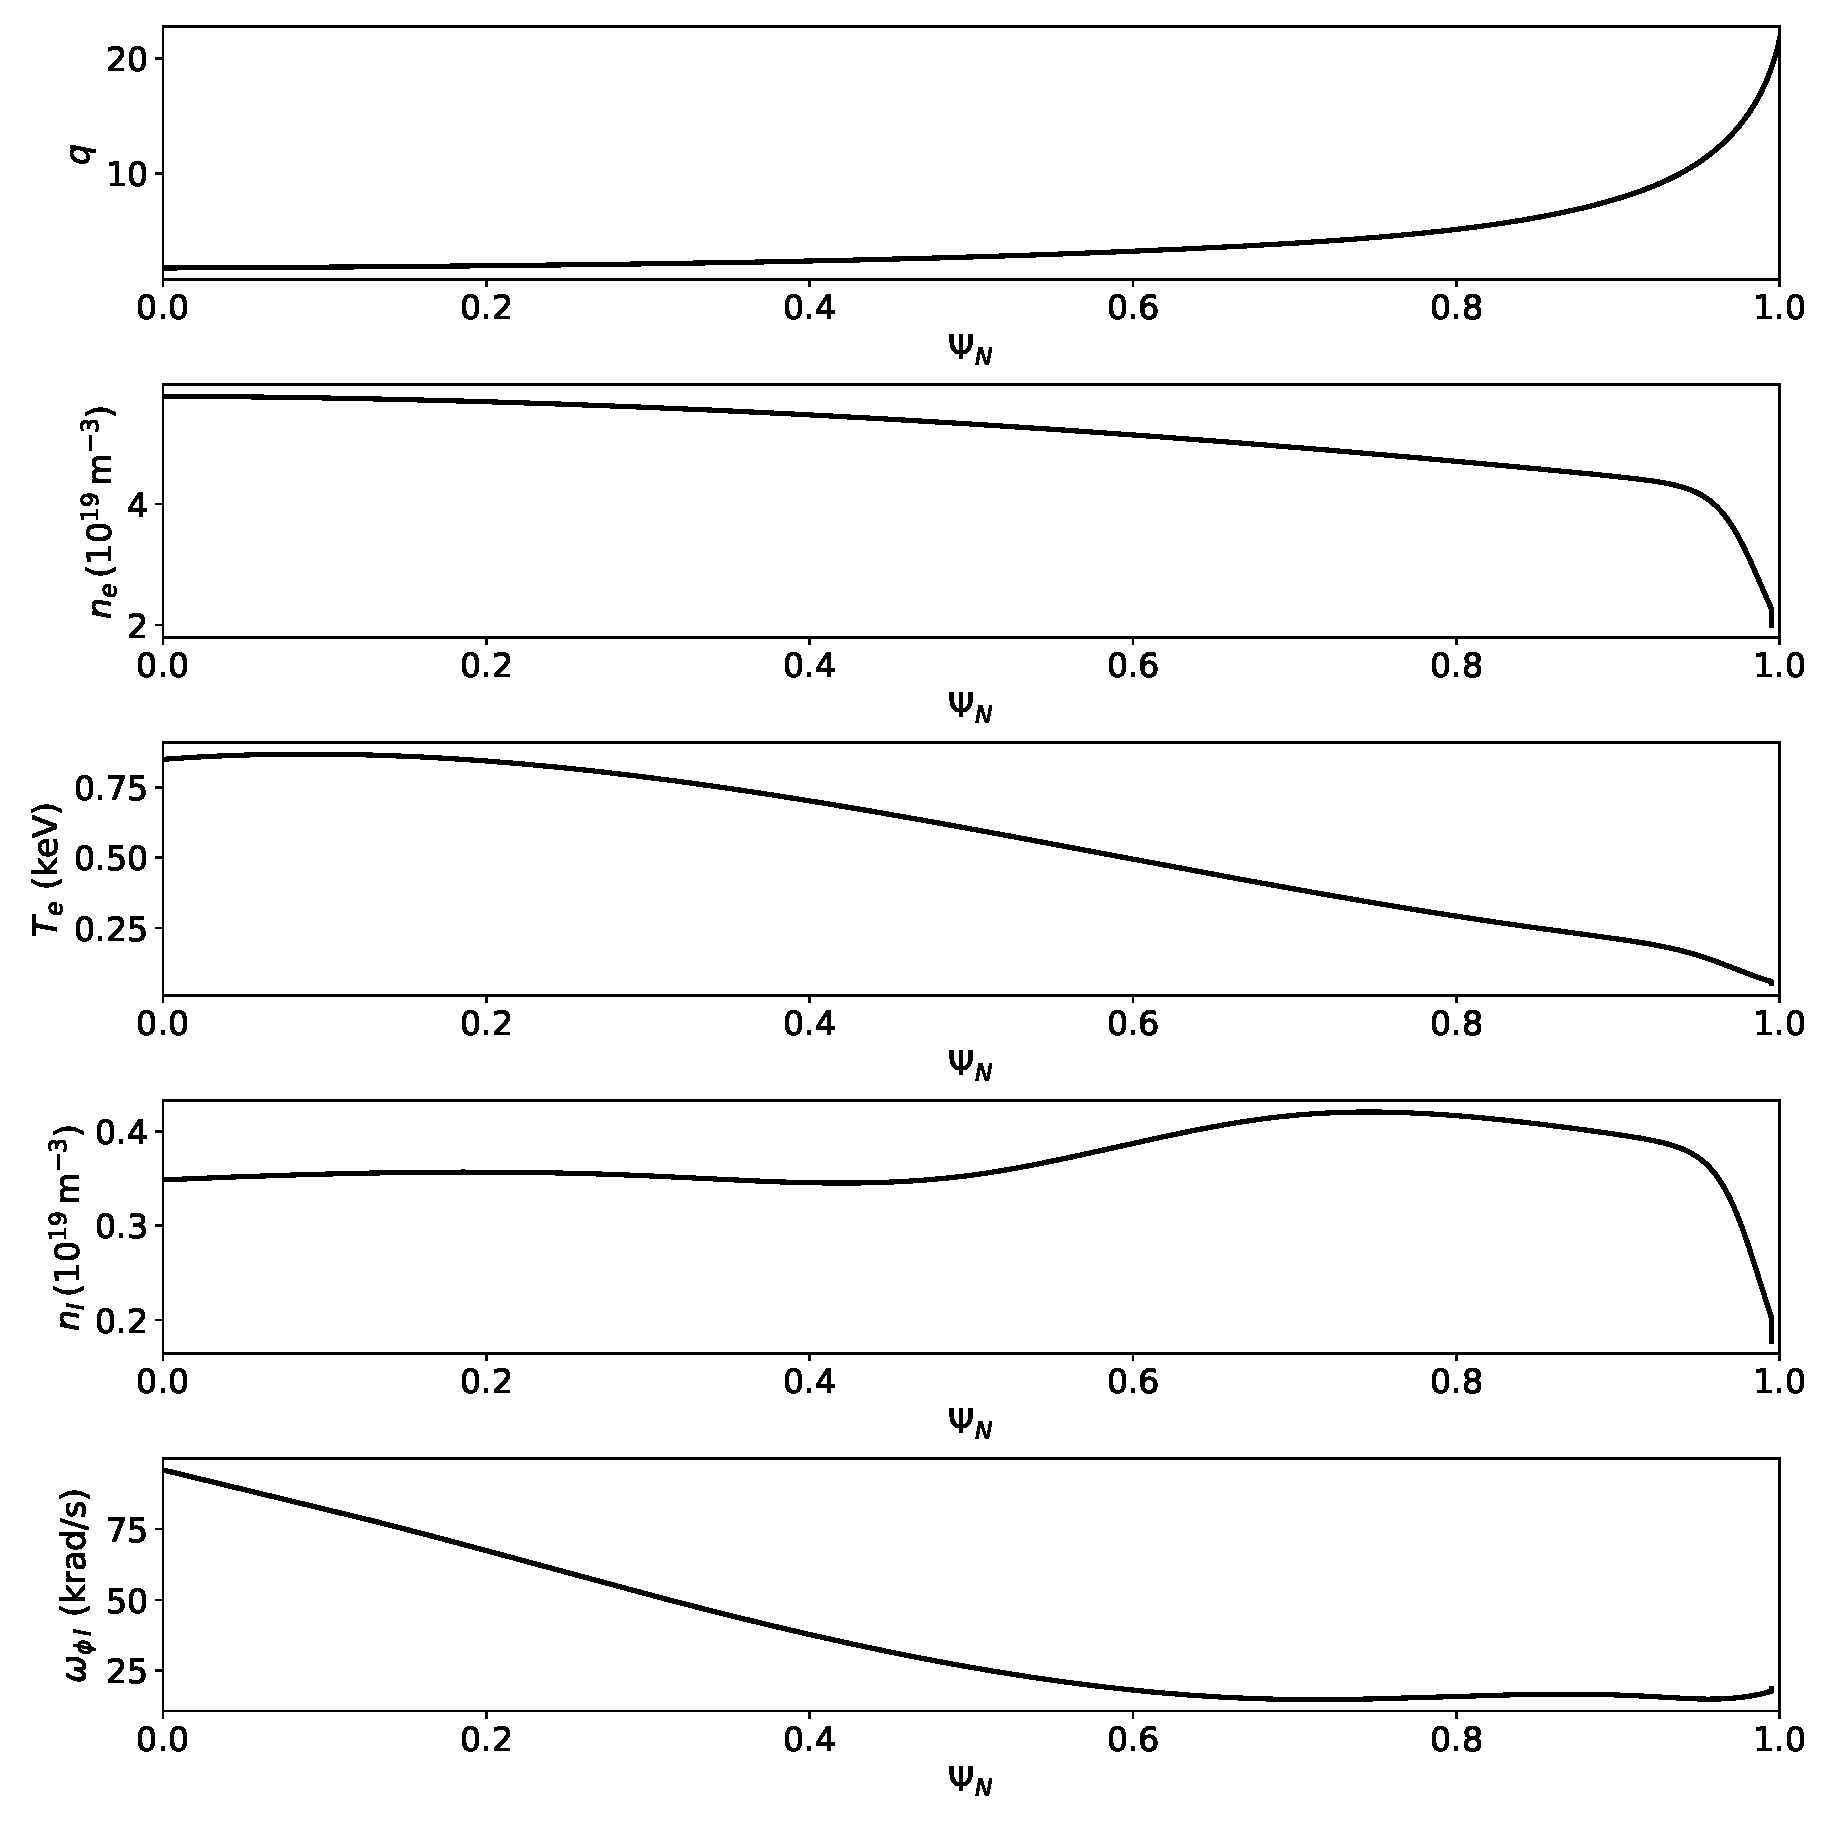
\includegraphics[height=6.25in]{Fig1.eps}}
\caption{Equilibrium magnetic flux-surfaces in NSTX discharge 127317 at $t=400$\, ms. Here, $R_0=0.85$ m.}\label{fig1}
\end{figure}

\begin{figure}
\centerline{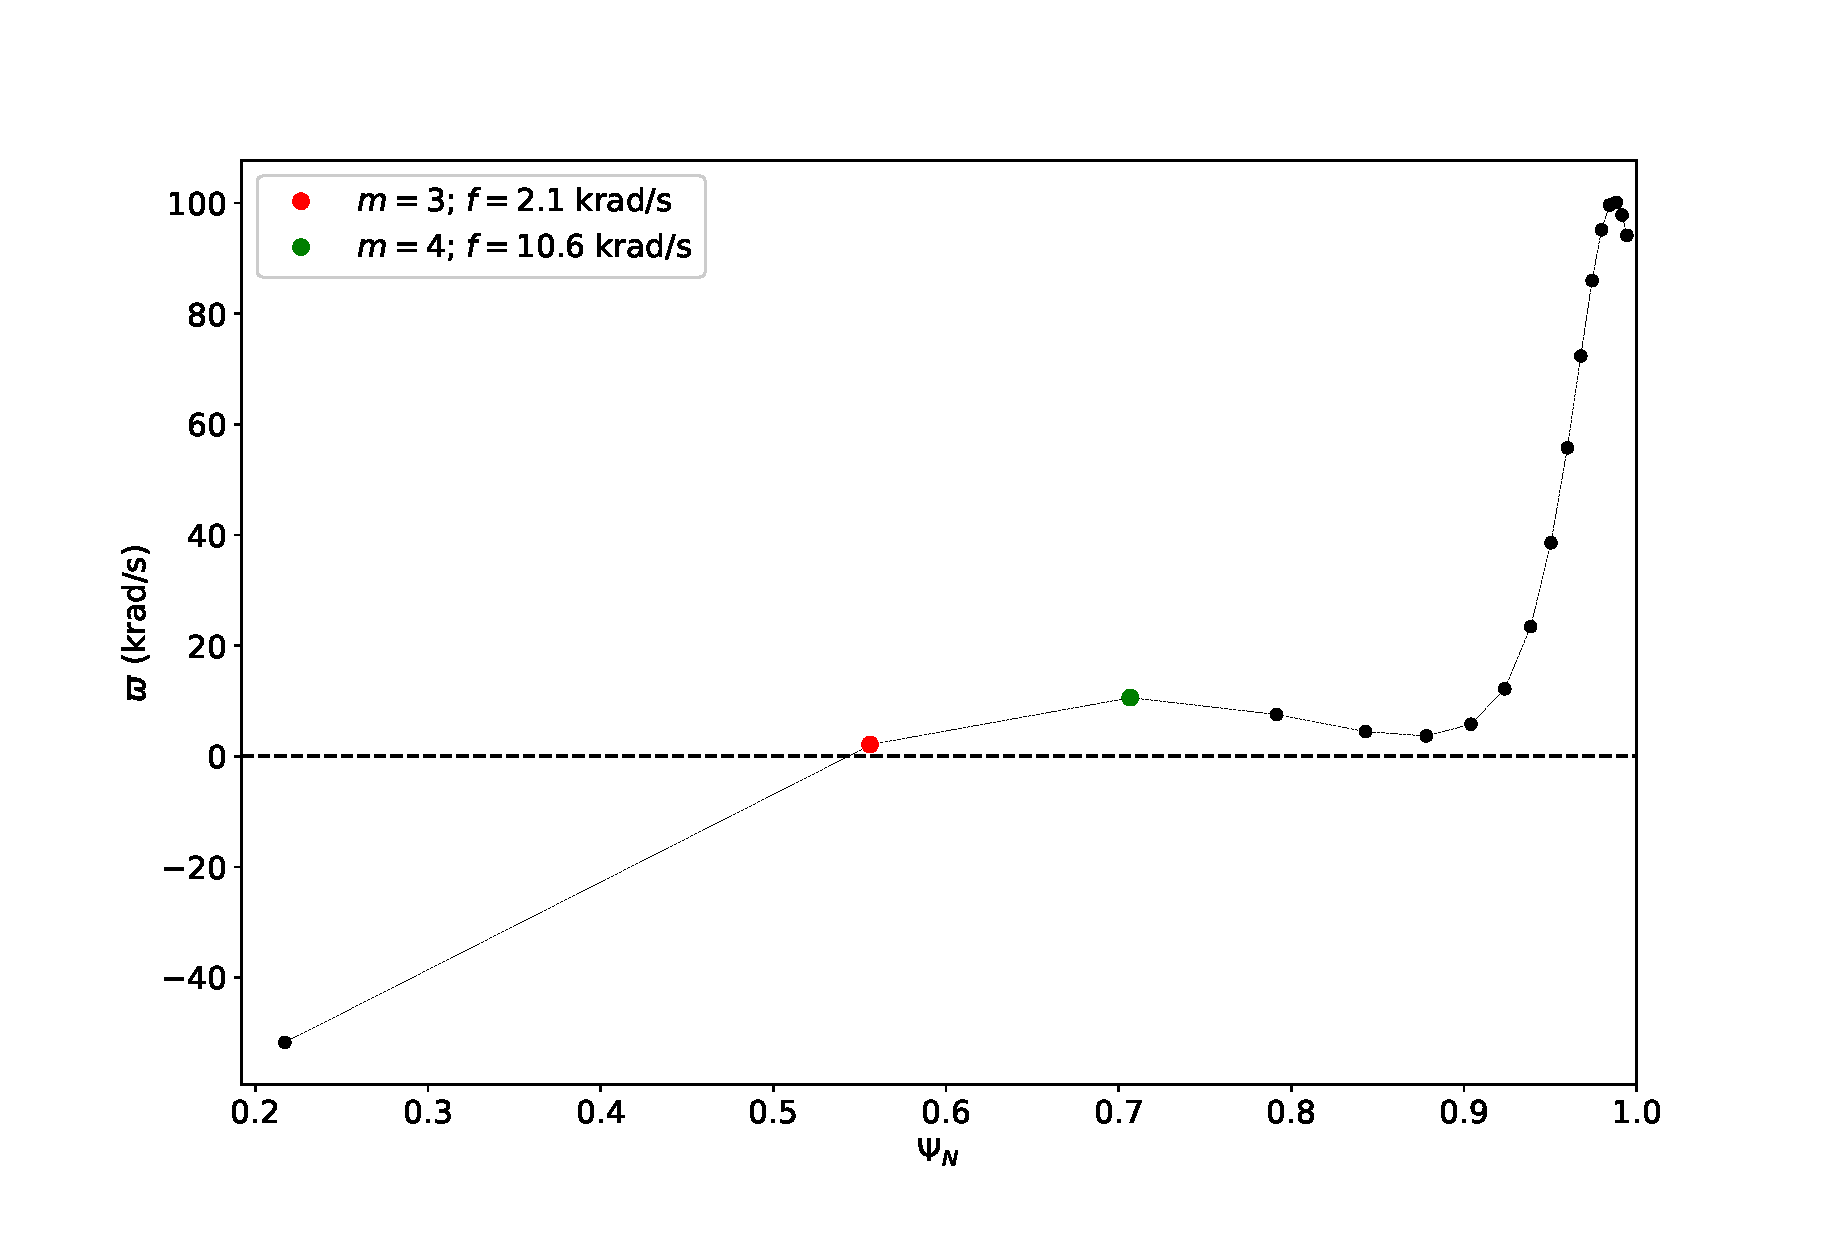
\includegraphics[height=6.25in]{Fig2.eps}}
\caption{The safety-factor, electron number density, electron temperature, impurity ion number density, and  impurity ion toroidal rotation profiles in NSTX discharge 127317 at $t=400$\, ms.}\label{fig2}
\end{figure}

\begin{figure}
\centerline{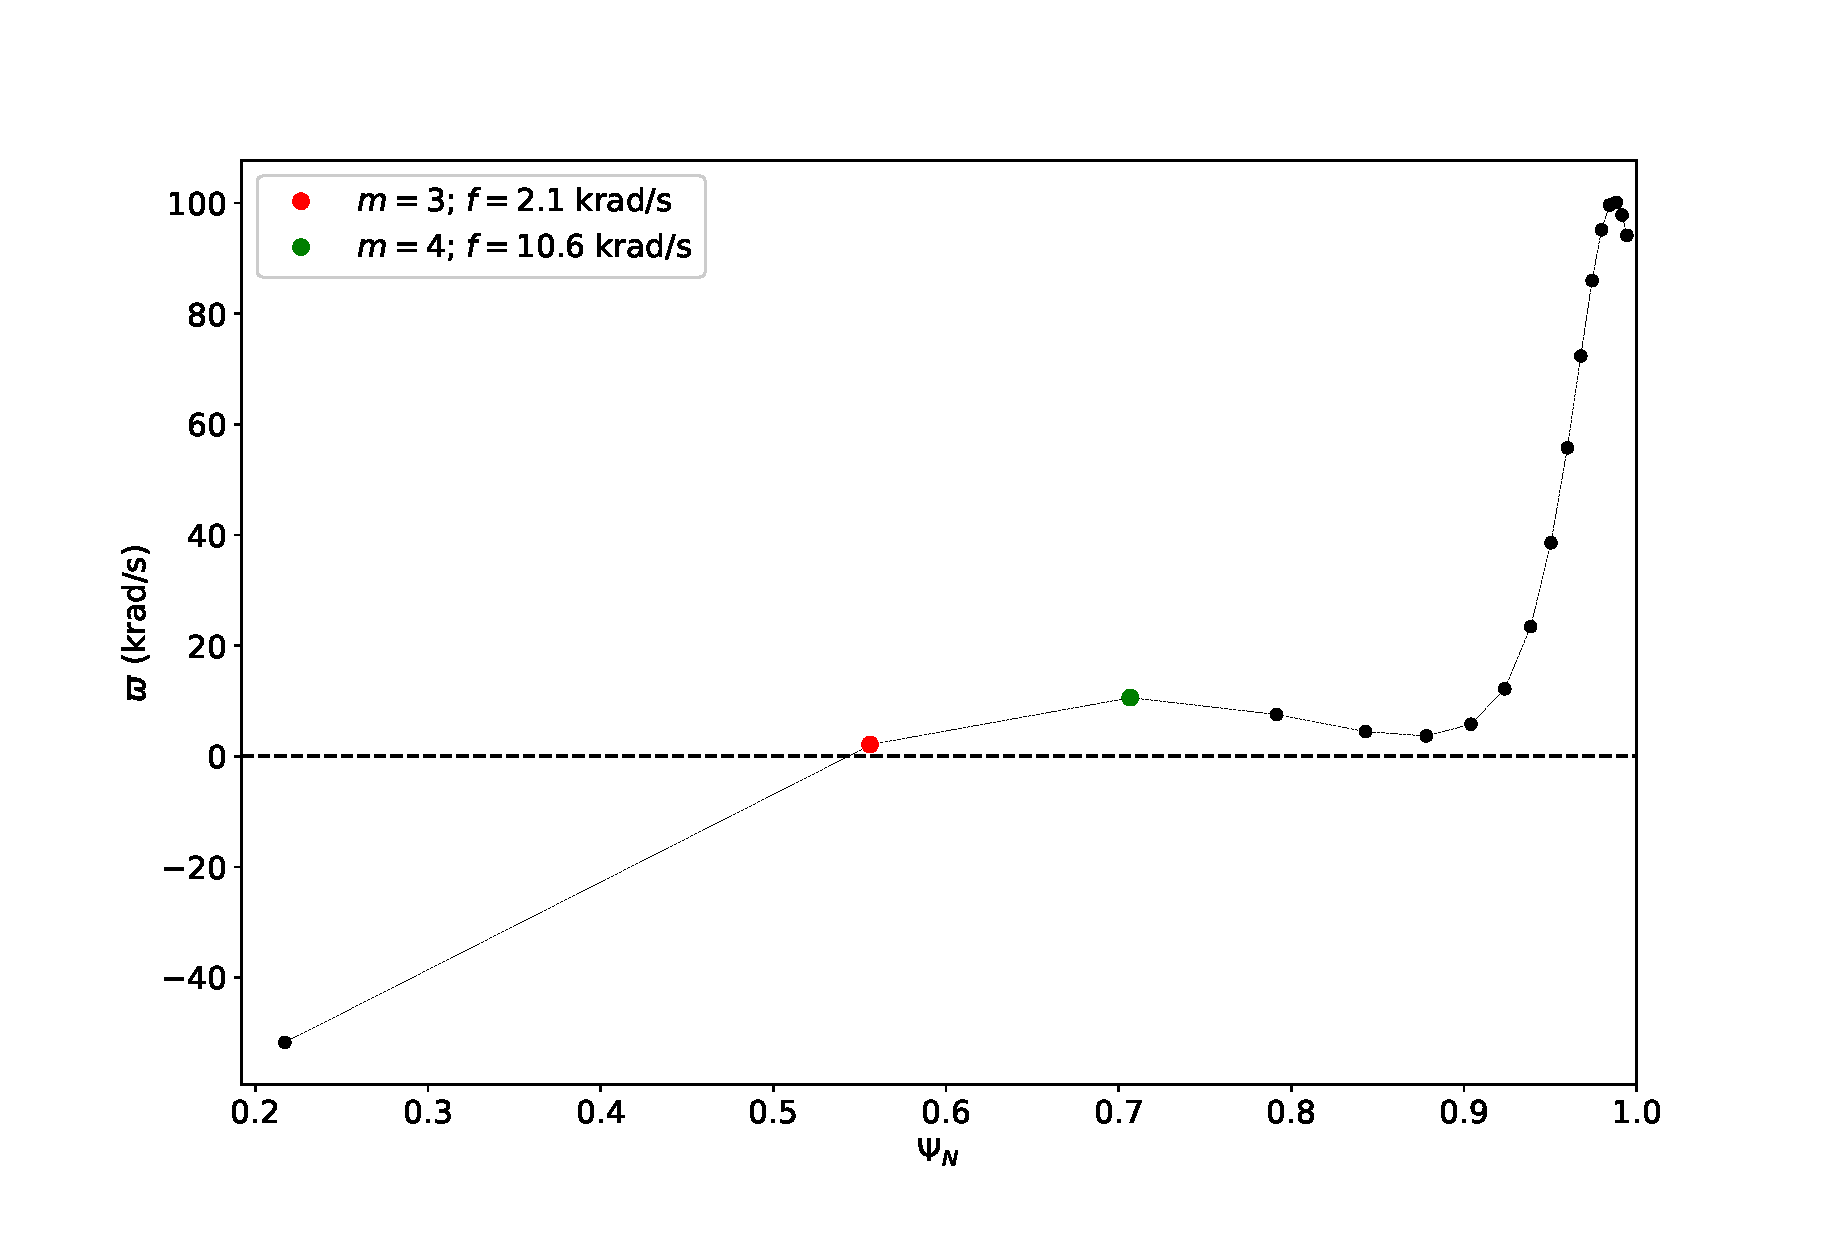
\includegraphics[height=5in]{Fig3.eps}}
\caption{Linear $n=1$ natural frequencies in NSTX discharge 127317 at $t=400$\, ms. There are 18 $n=1$ resonant surfaces in the plasma corresponding to $m=2$ through $m=19$. Only the $m=3$ and $m=4$ surfaces are potentially
unstable to NTMs.}\label{fig3}
\end{figure}

\begin{figure}
\centerline{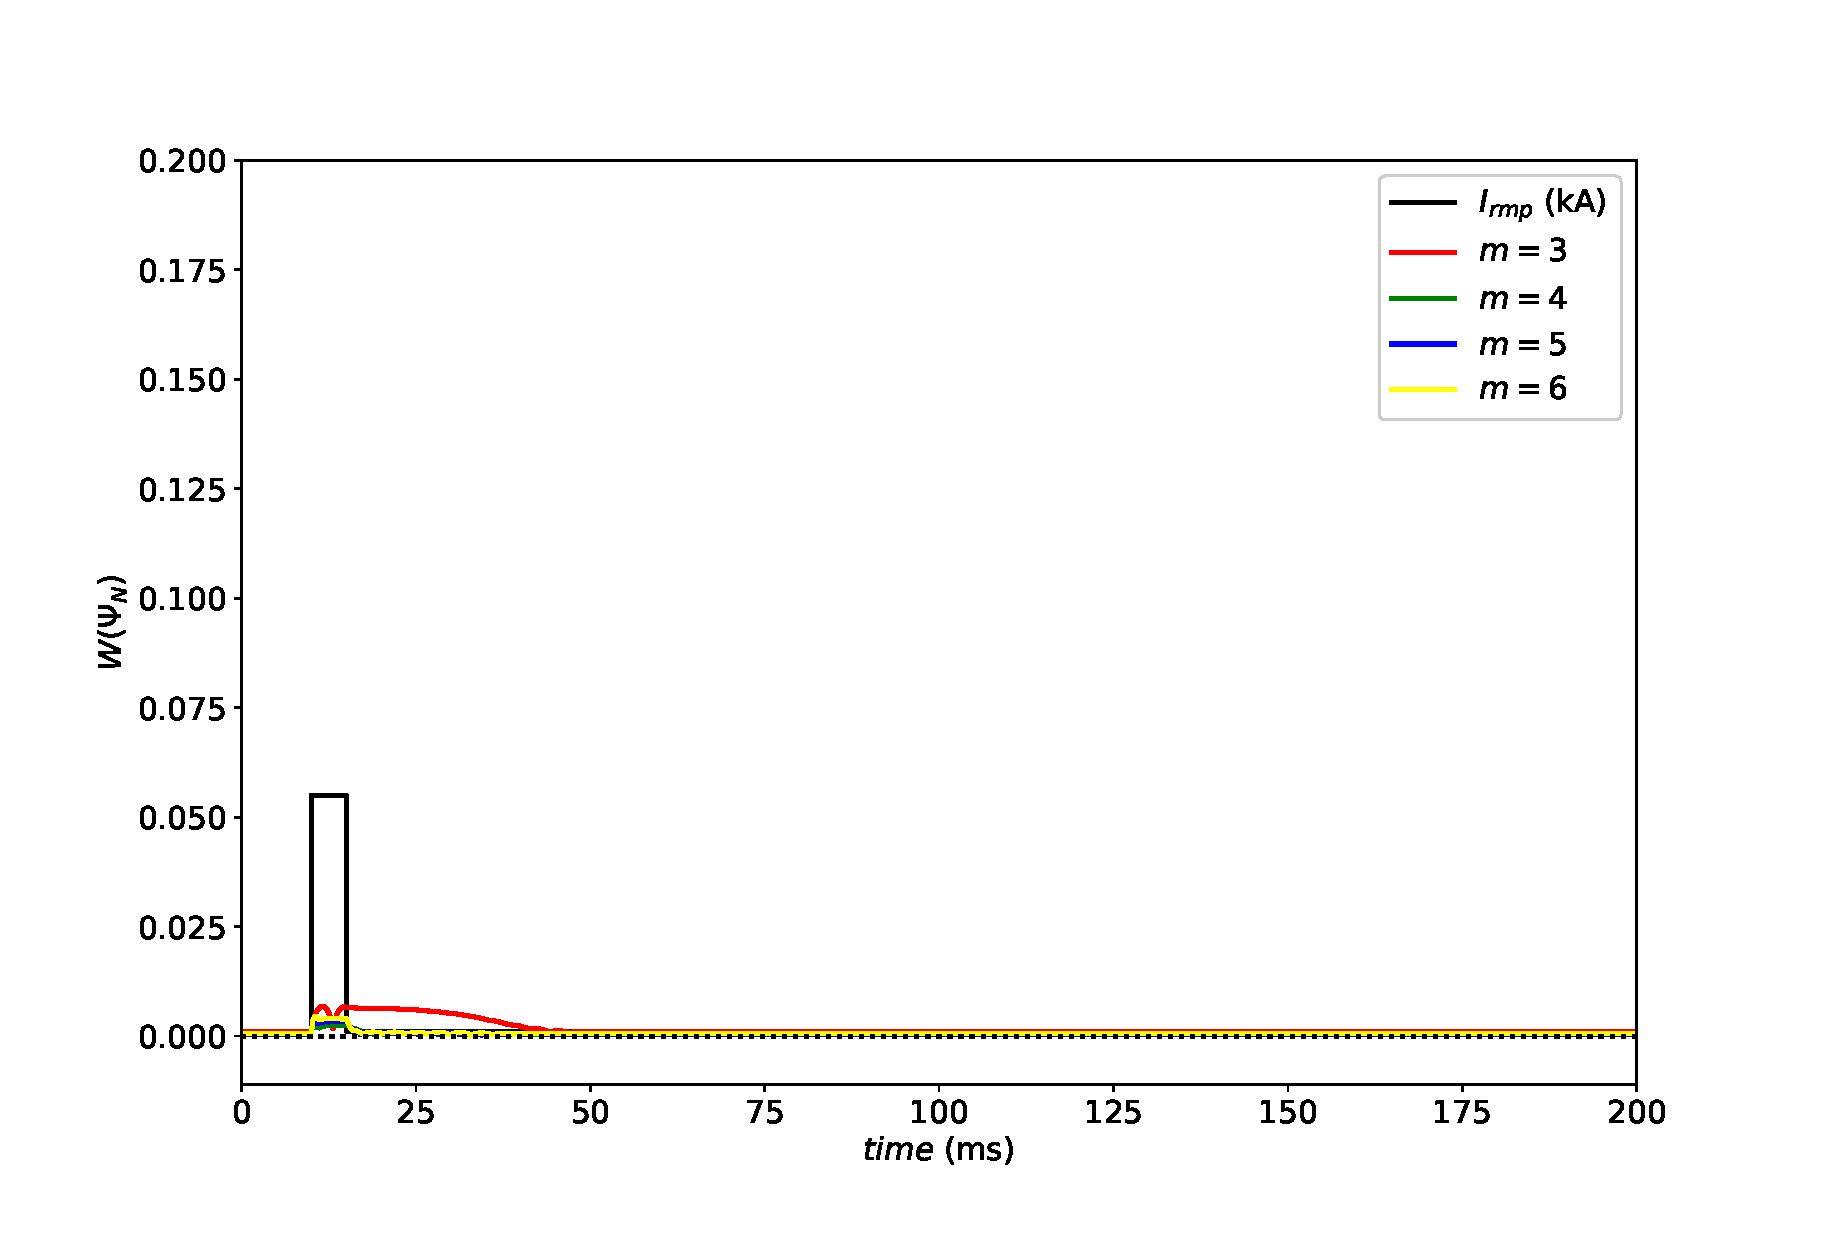
\includegraphics[height=6in]{Fig4.eps}}
\caption{Right-hand sides of modified Rutherford equations for $m=3/n=1$ and $m=4/n=1$ tearing modes in NSTX discharge 127317 at $t=400$\, ms.}\label{fig4}
\end{figure}

\begin{figure}
\centerline{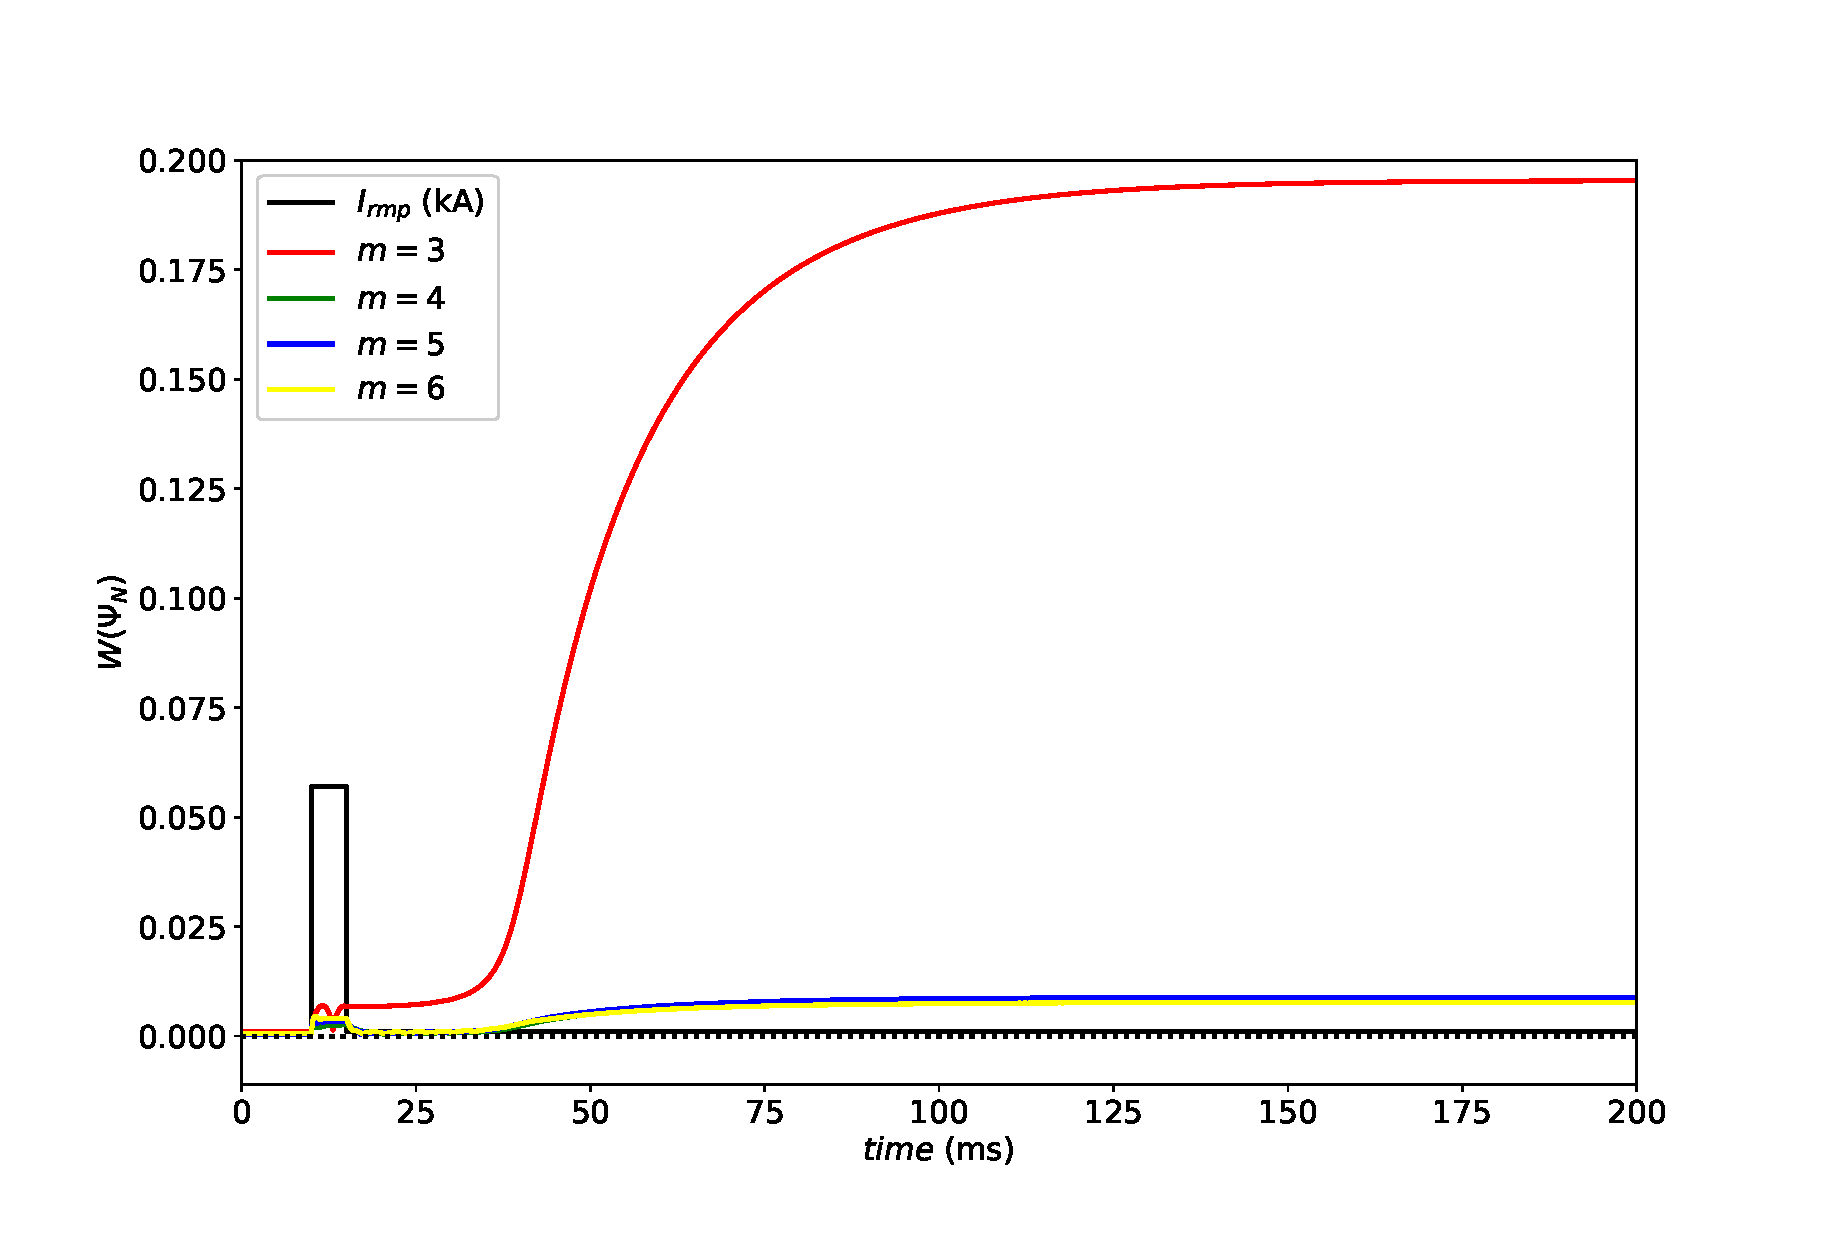
\includegraphics[height=5in]{Fig5.eps}}
\caption{Calculated $n=1$ island widths  versus time in NSTX discharge 127317 in response to an $n=1$ current pulse of amplitude $0.055$ kA, duration 5 ms, and frequency 0 krad/s applied to the RMP coils.}\label{fig5}
\end{figure}

\begin{figure}
\centerline{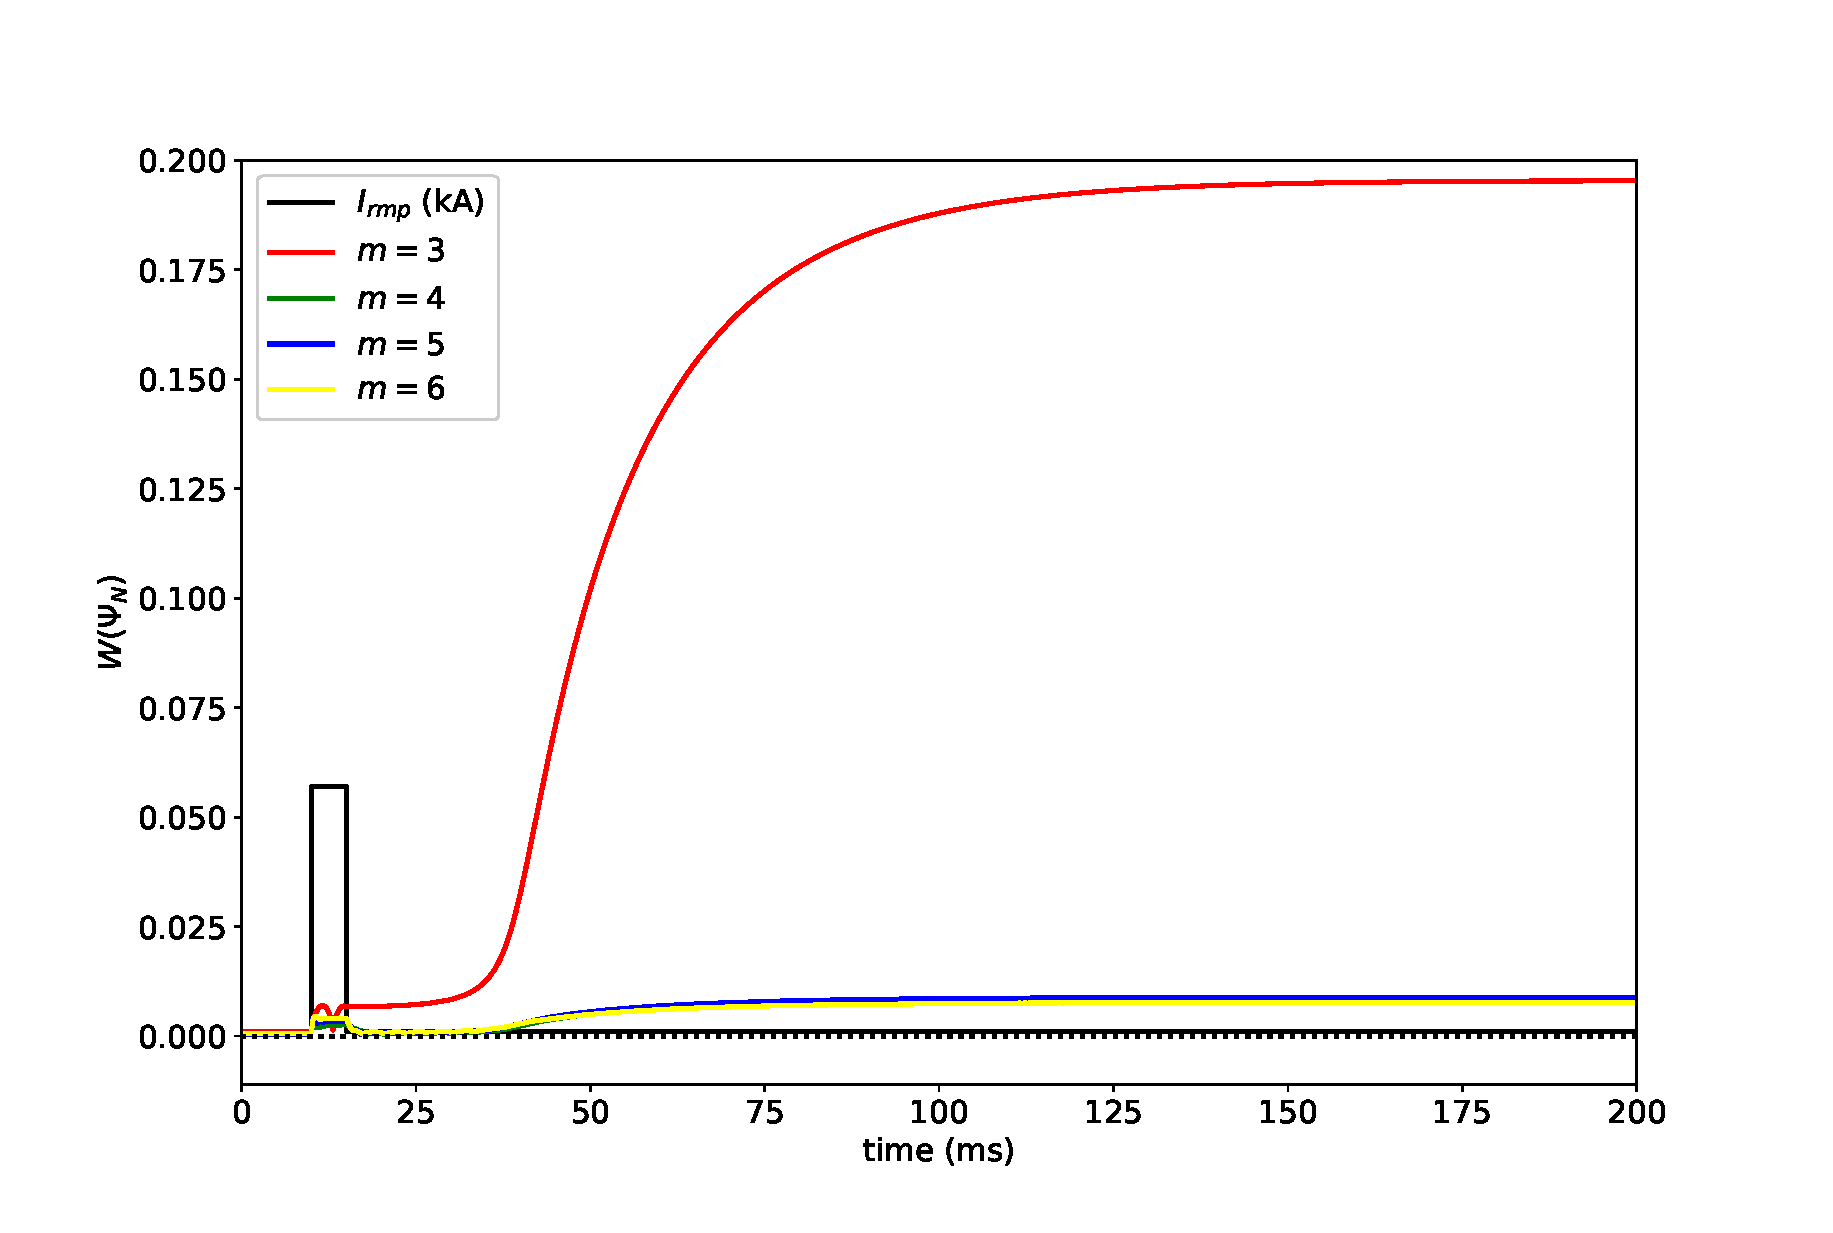
\includegraphics[height=5in]{Fig6.eps}}
\caption{Calculated $n=1$ island widths versus time in NSTX discharge 127317 in response to an $n=1$ current pulse of amplitude $0.057$ kA, duration 5 ms, and frequency 0 krad/s applied to the RMP coils.}\label{fig6}
\end{figure}

\begin{figure}
\centerline{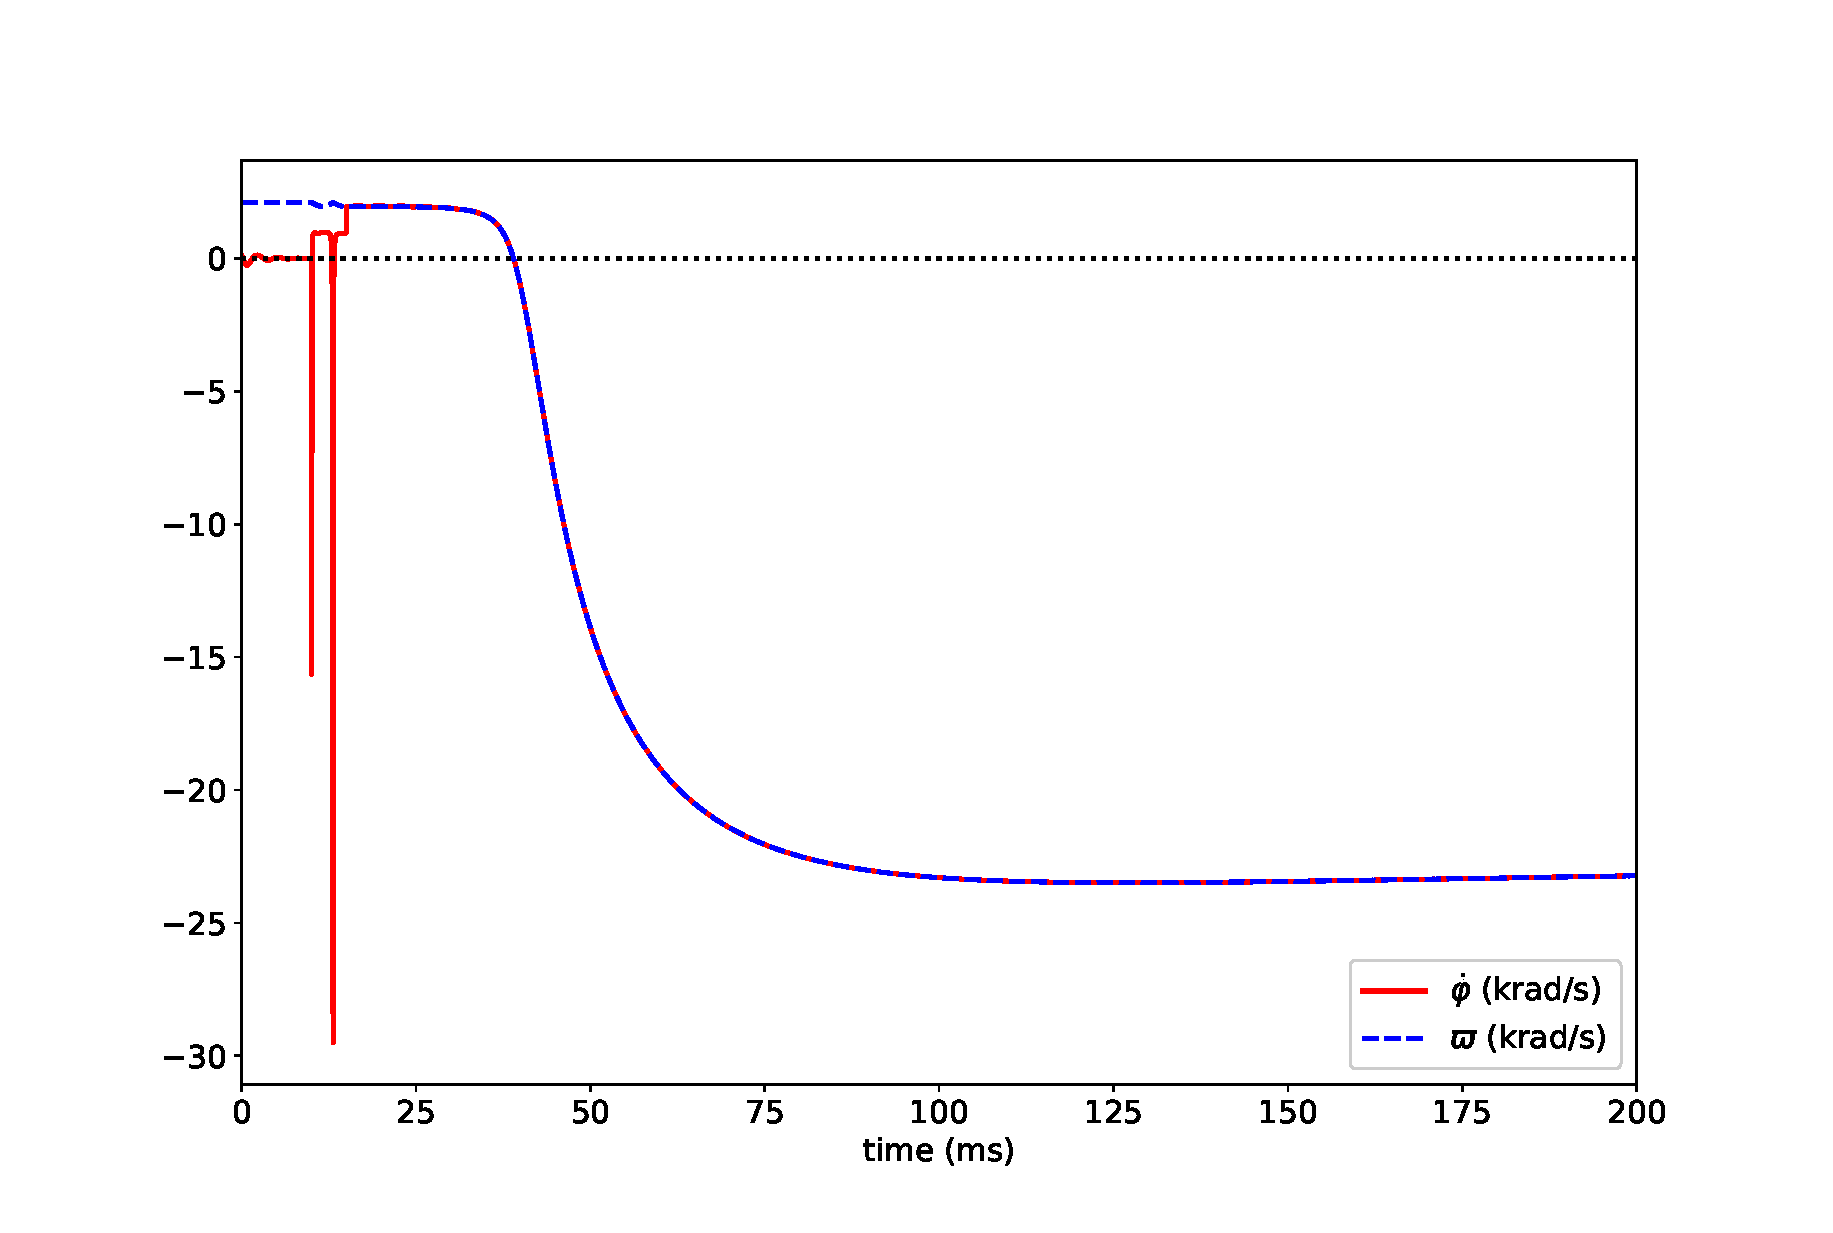
\includegraphics[height=5in]{Fig7.eps}}
\caption{Calculated phase velocity ($\dot{\varphi}$) and natural frequency ($\varpi$) of $m=3/n=1$ mode versus time in NSTX discharge 127317 in response to an $n=1$ current pulse of amplitude $0.057$ kA, duration 5 ms, and frequency 0 krad/s applied to the RMP coils.}\label{fig7}
\end{figure}

\begin{figure}
\centerline{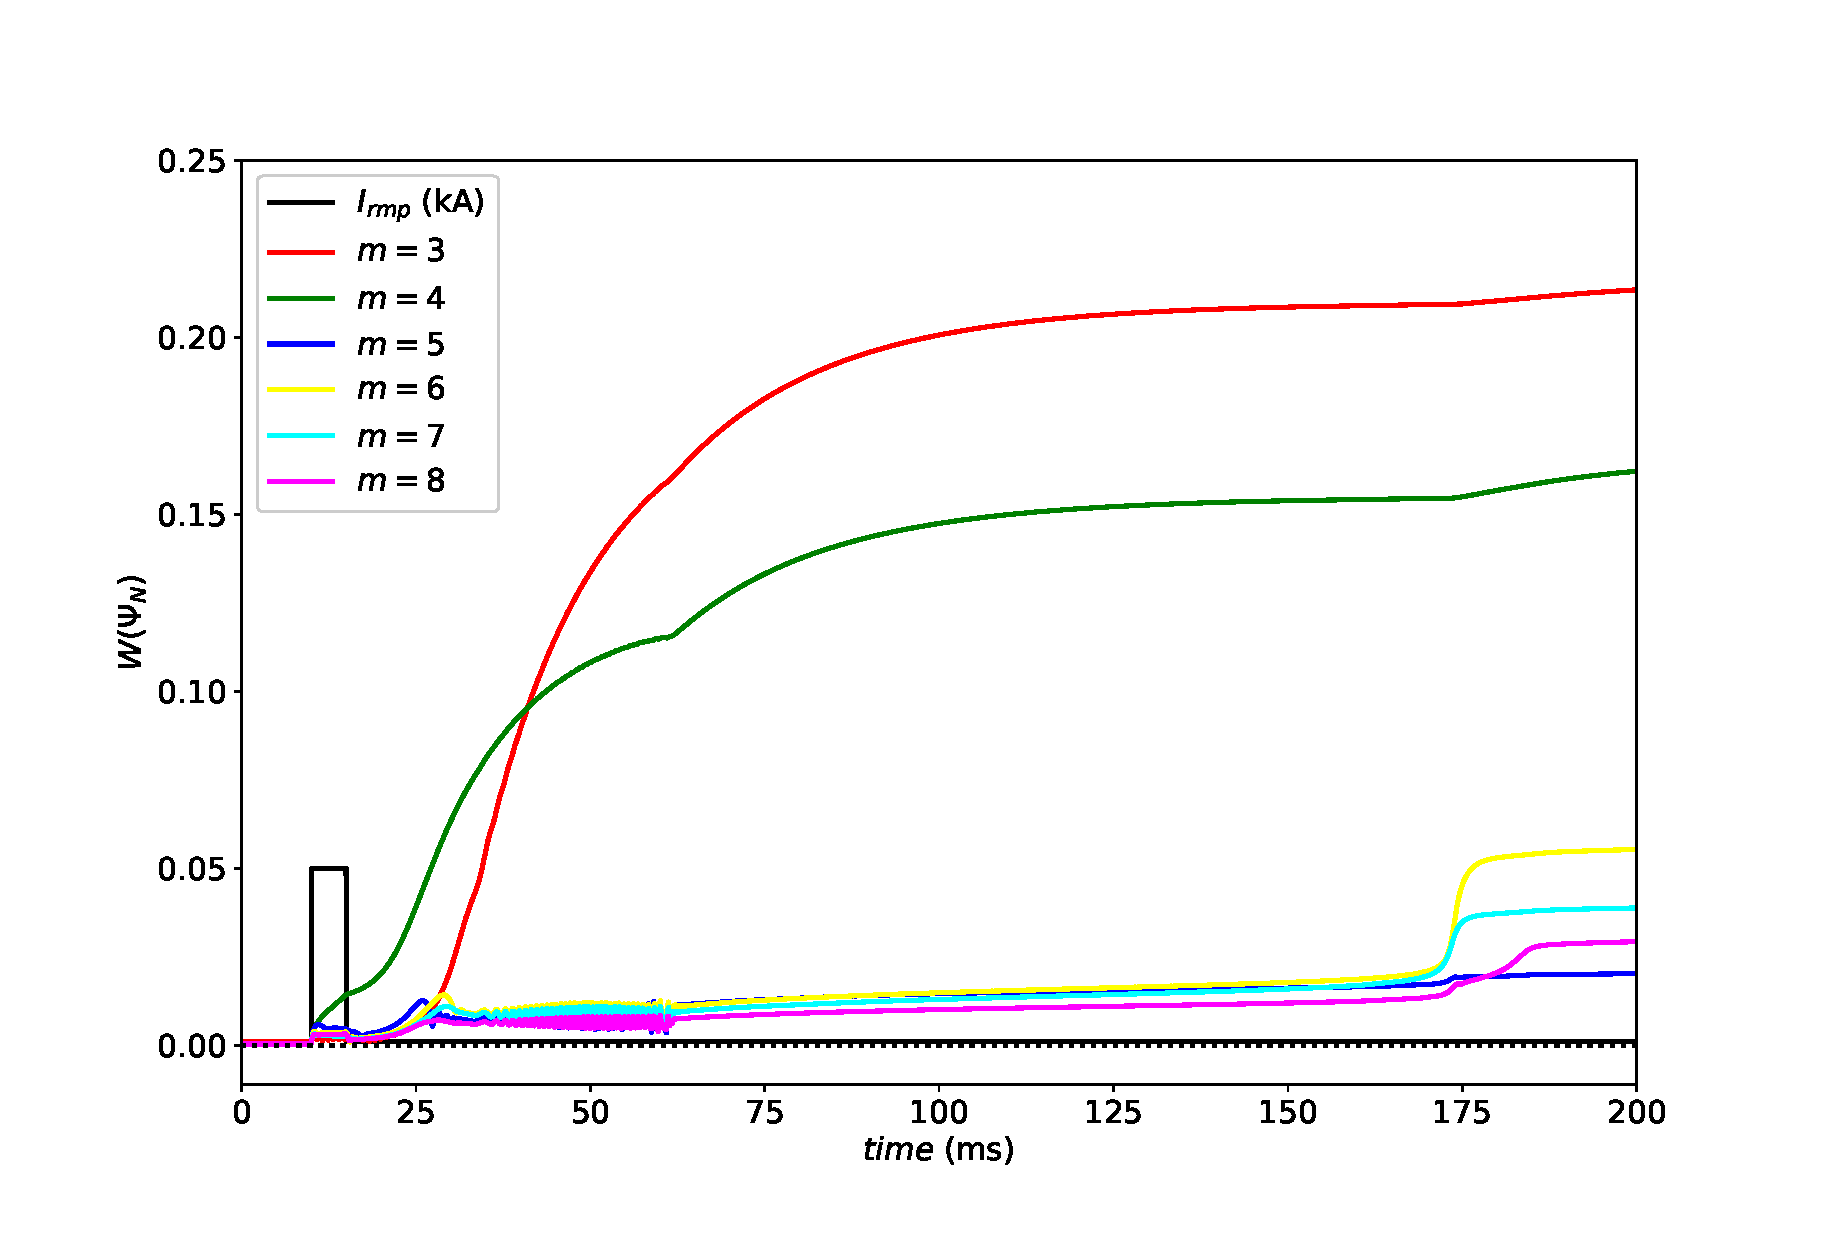
\includegraphics[height=5in]{Fig8.eps}}
\caption{Critical $n=1$ RMP coil current pulse amplitude required to trigger an $m=3/n=1$ NTM in NSTX discharge 127317 
as a function of the pulse duration  for various different pulse frequencies.}\label{fig8}
\end{figure}

\begin{figure}
\centerline{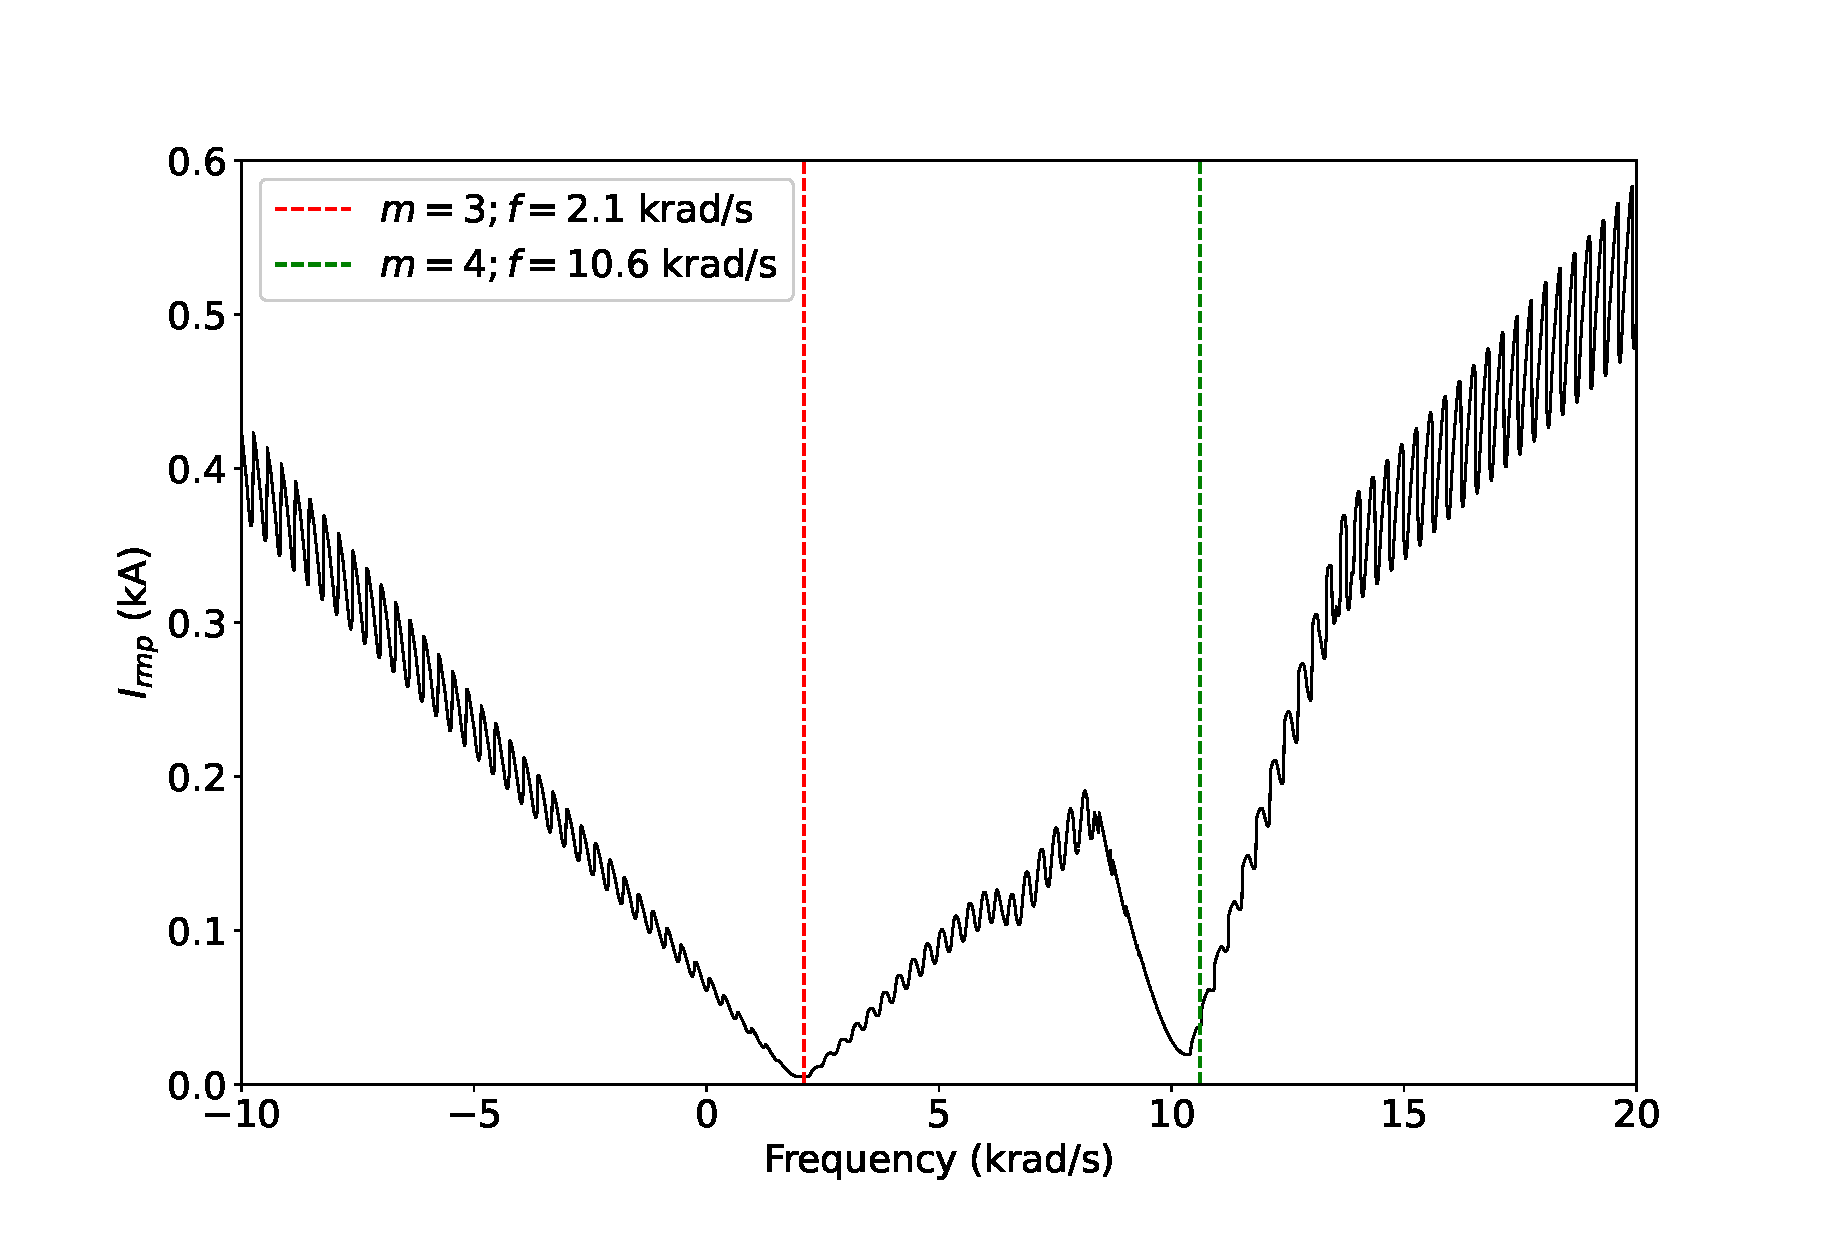
\includegraphics[height=5in]{Fig9.eps}}
\caption{Critical $n=1$ RMP coil current pulse amplitude required to trigger an $m=3/n=1$ NTM in NSTX discharge 127317 
as a function of the pulse frequency for a pulse duration of 20 ms.}\label{fig9}
\end{figure}

\begin{figure}
\centerline{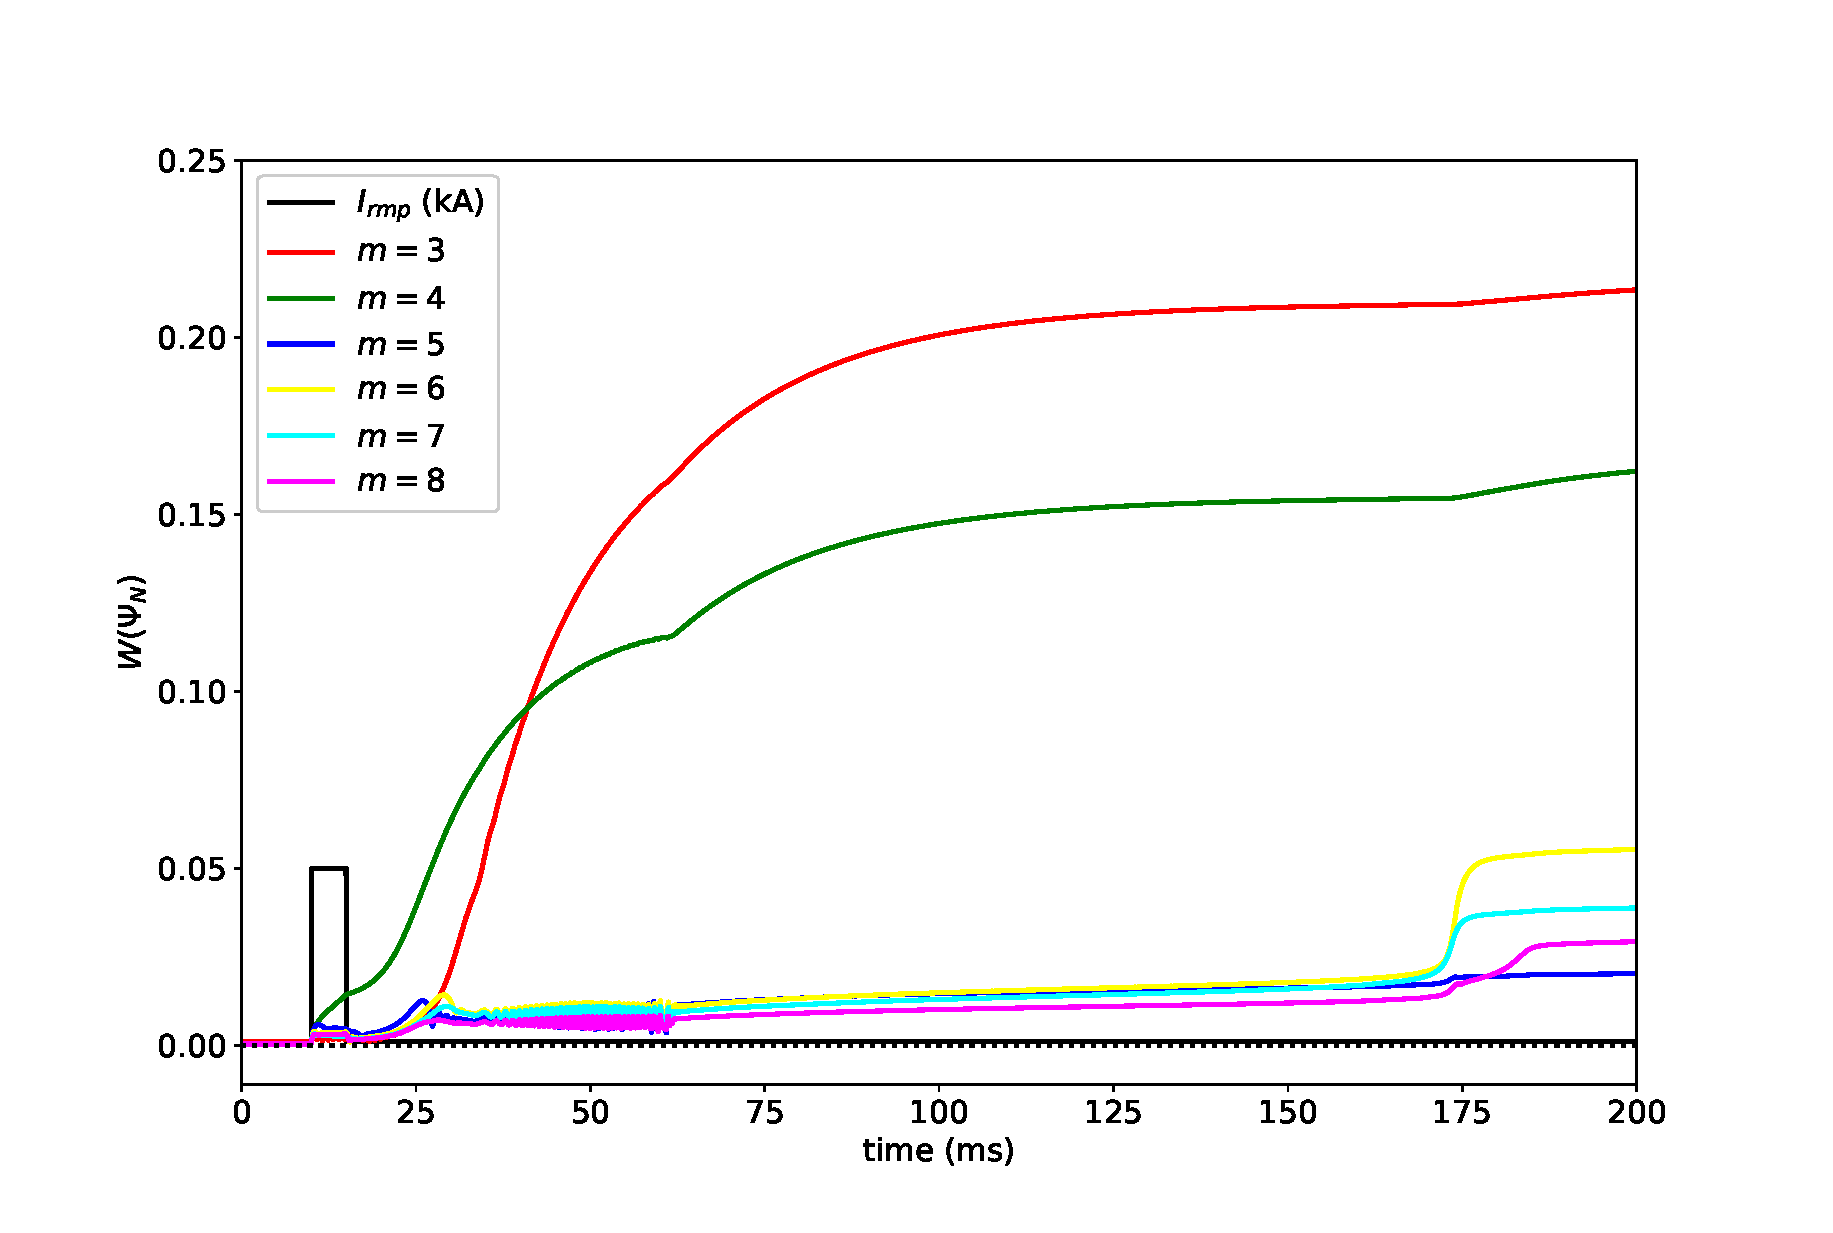
\includegraphics[height=5in]{Fig10.eps}}
\caption{Calculated $n=1$ island widths versus time in NSTX discharge 127317 in response to an $n=1$ current pulse of amplitude $0.05$ kA, duration 5 ms, and frequency 10 krad/s applied to the RMP coils.}\label{fig10}
\end{figure}

\begin{figure}
\centerline{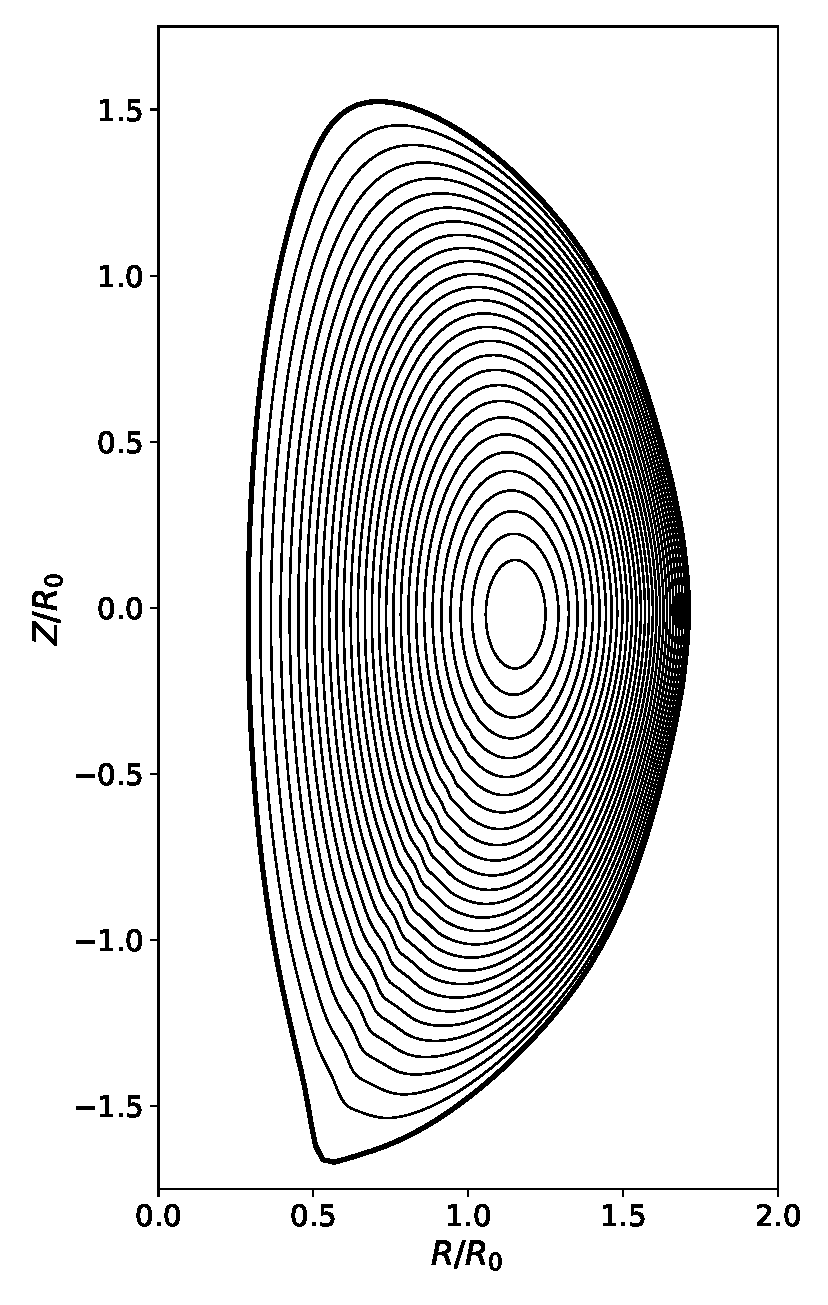
\includegraphics[height=6.25in]{Fig11.eps}}
\caption{Equilibrium magnetic flux-surfaces in NSTX discharge  139057 at $t=557$\, ms. Here, $R_0=0.85$ m.}\label{fig11}
\end{figure}

\begin{figure}
\centerline{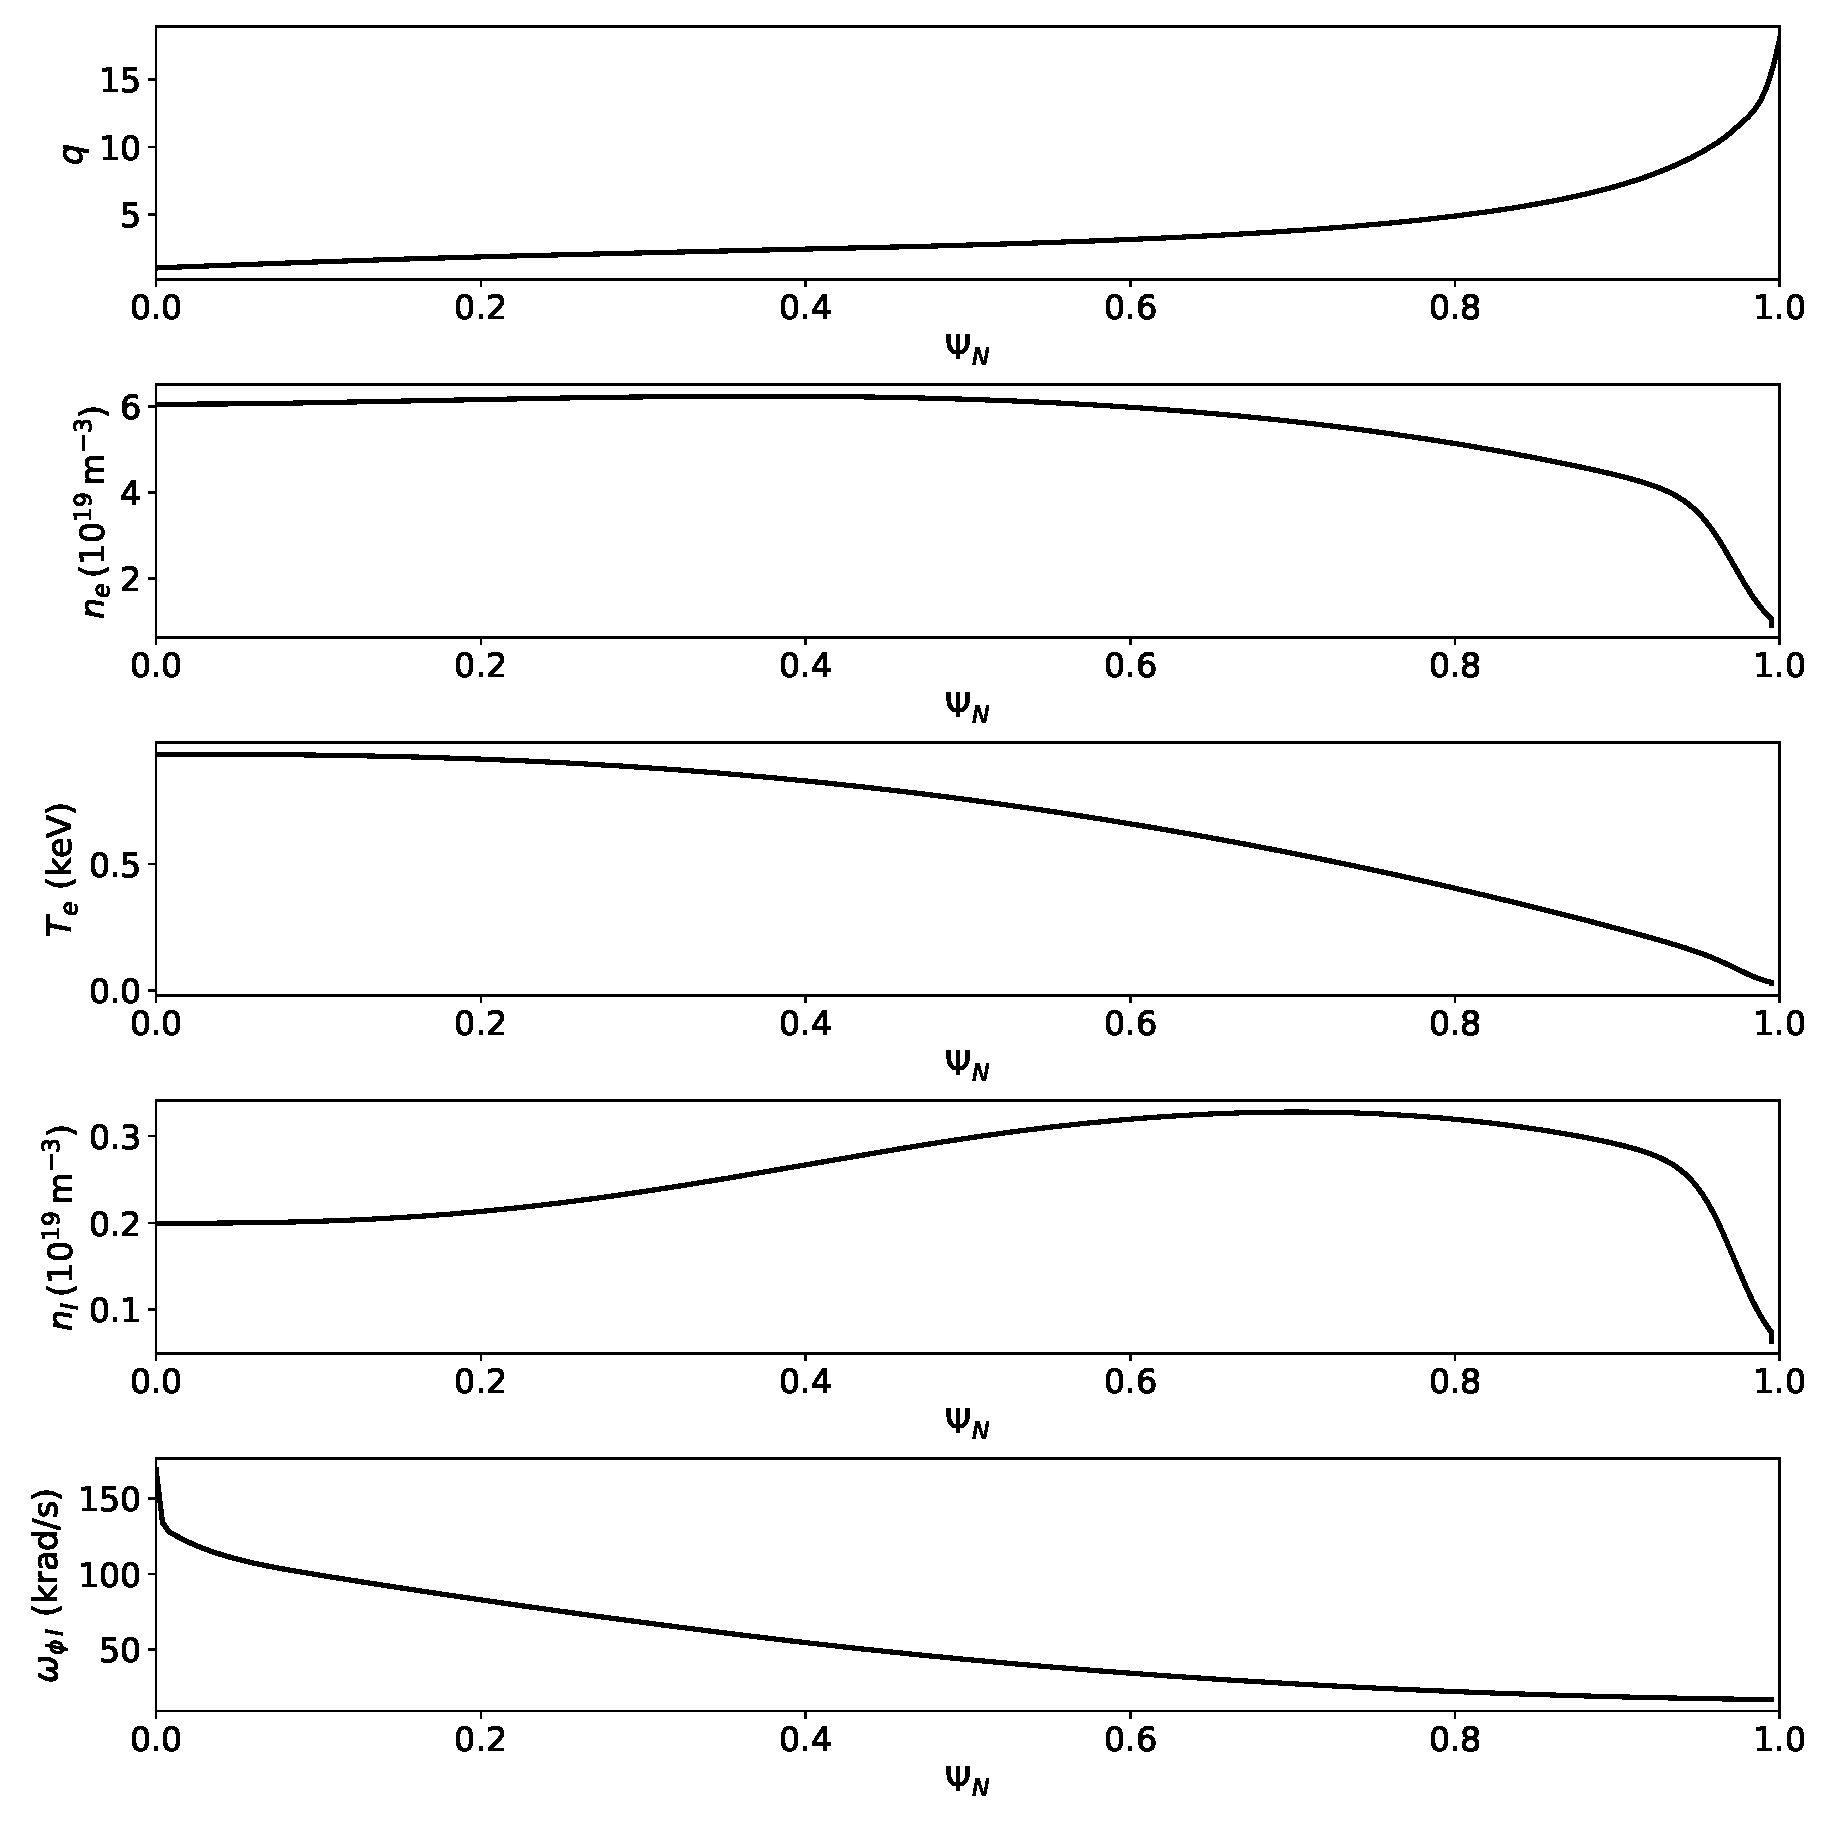
\includegraphics[height=6.25in]{Fig12.eps}}
\caption{The safety-factor, electron number density, electron temperature, impurity ion number density, and  impurity ion toroidal rotation profiles in NSTX discharge 139057 at $t=557$\, ms.}\label{fig12}
\end{figure}

\begin{figure}
\centerline{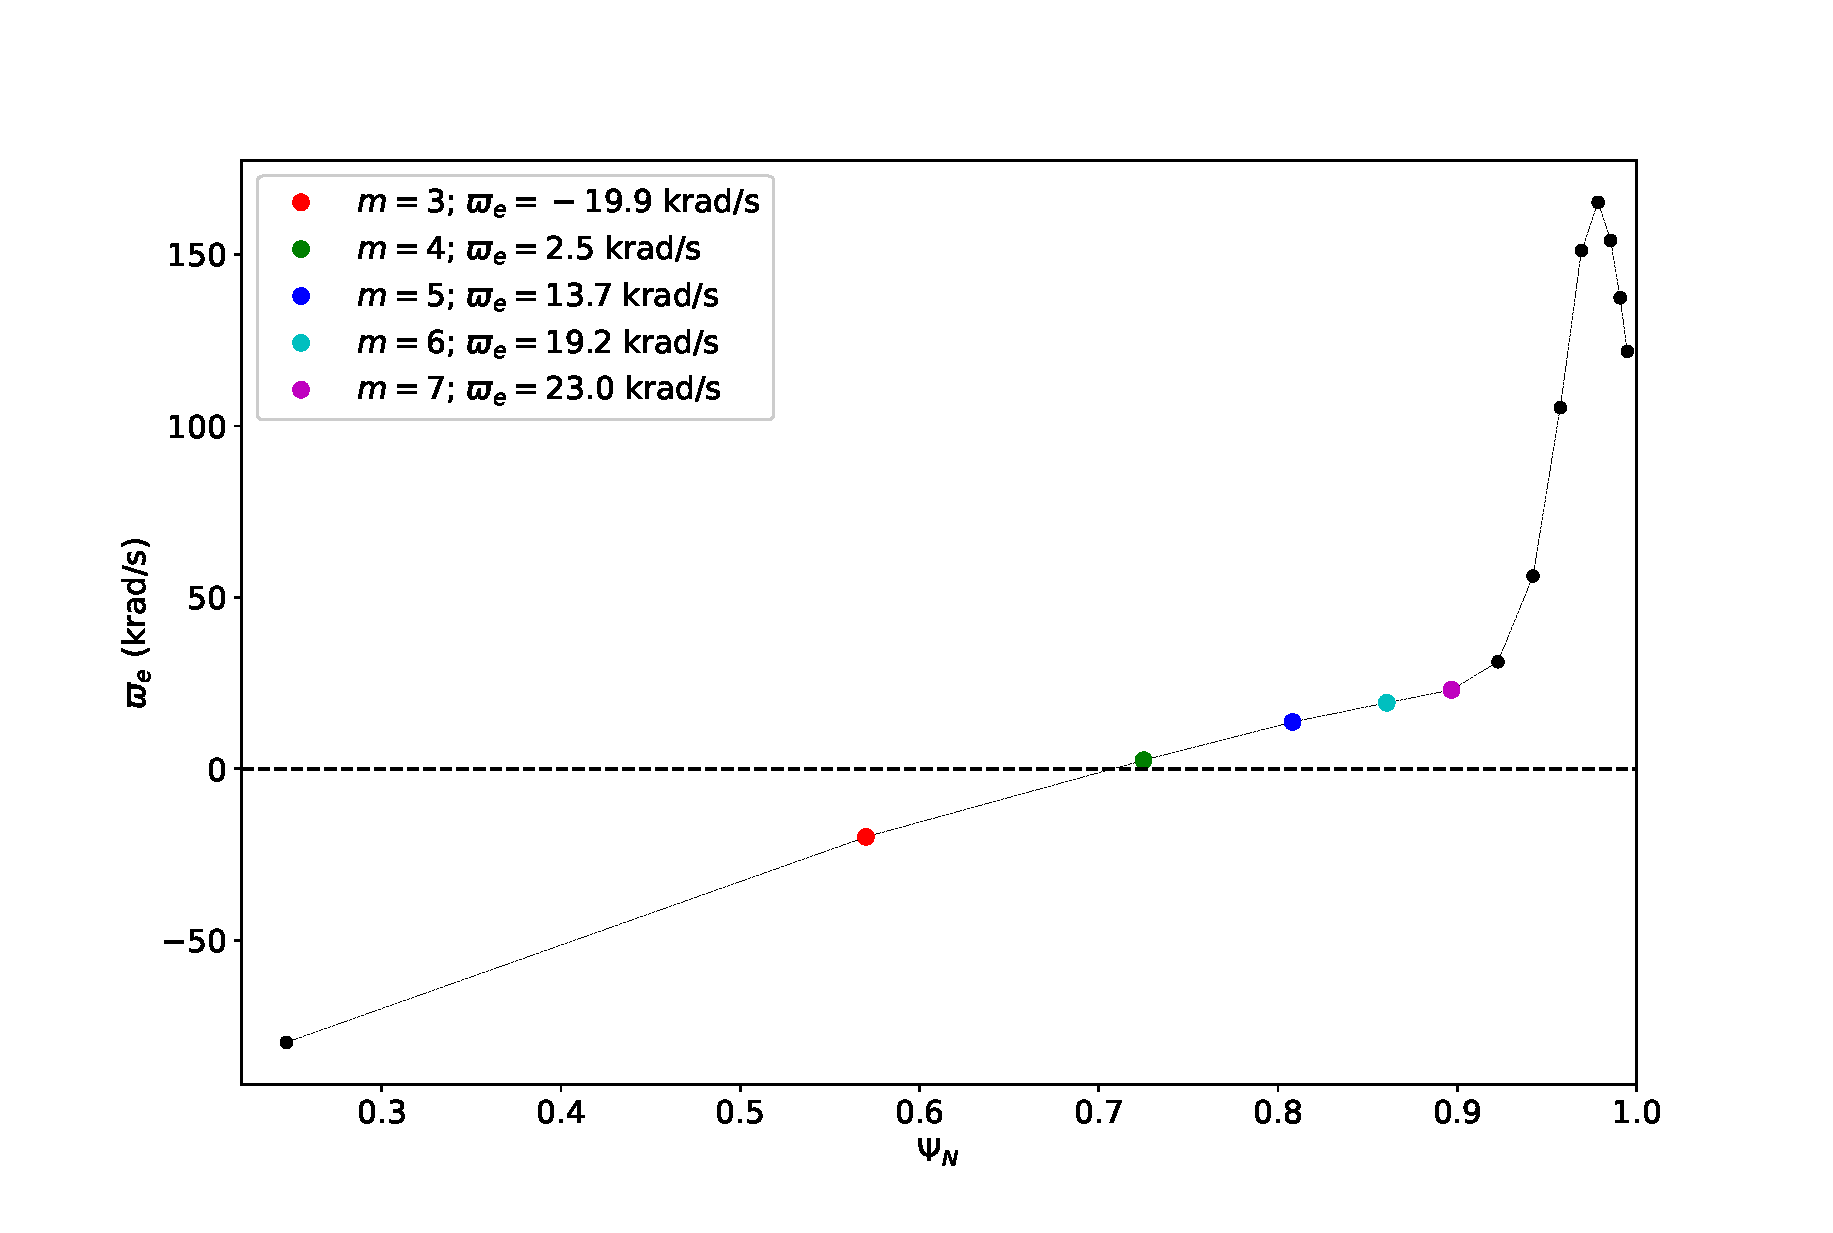
\includegraphics[height=5in]{Fig13.eps}}
\caption{Linear $n=1$ natural frequencies in NSTX discharge 139057 at $t=557$\, ms. There are 14 $n=1$ resonant surfaces in the plasma corresponding to $m=2$ through $m=15$. Only the $m=3$, $4$, $5$, $6$, and $7$ surfaces are potentially
unstable to NTMs.}\label{fig13}
\end{figure}

\begin{figure}
\centerline{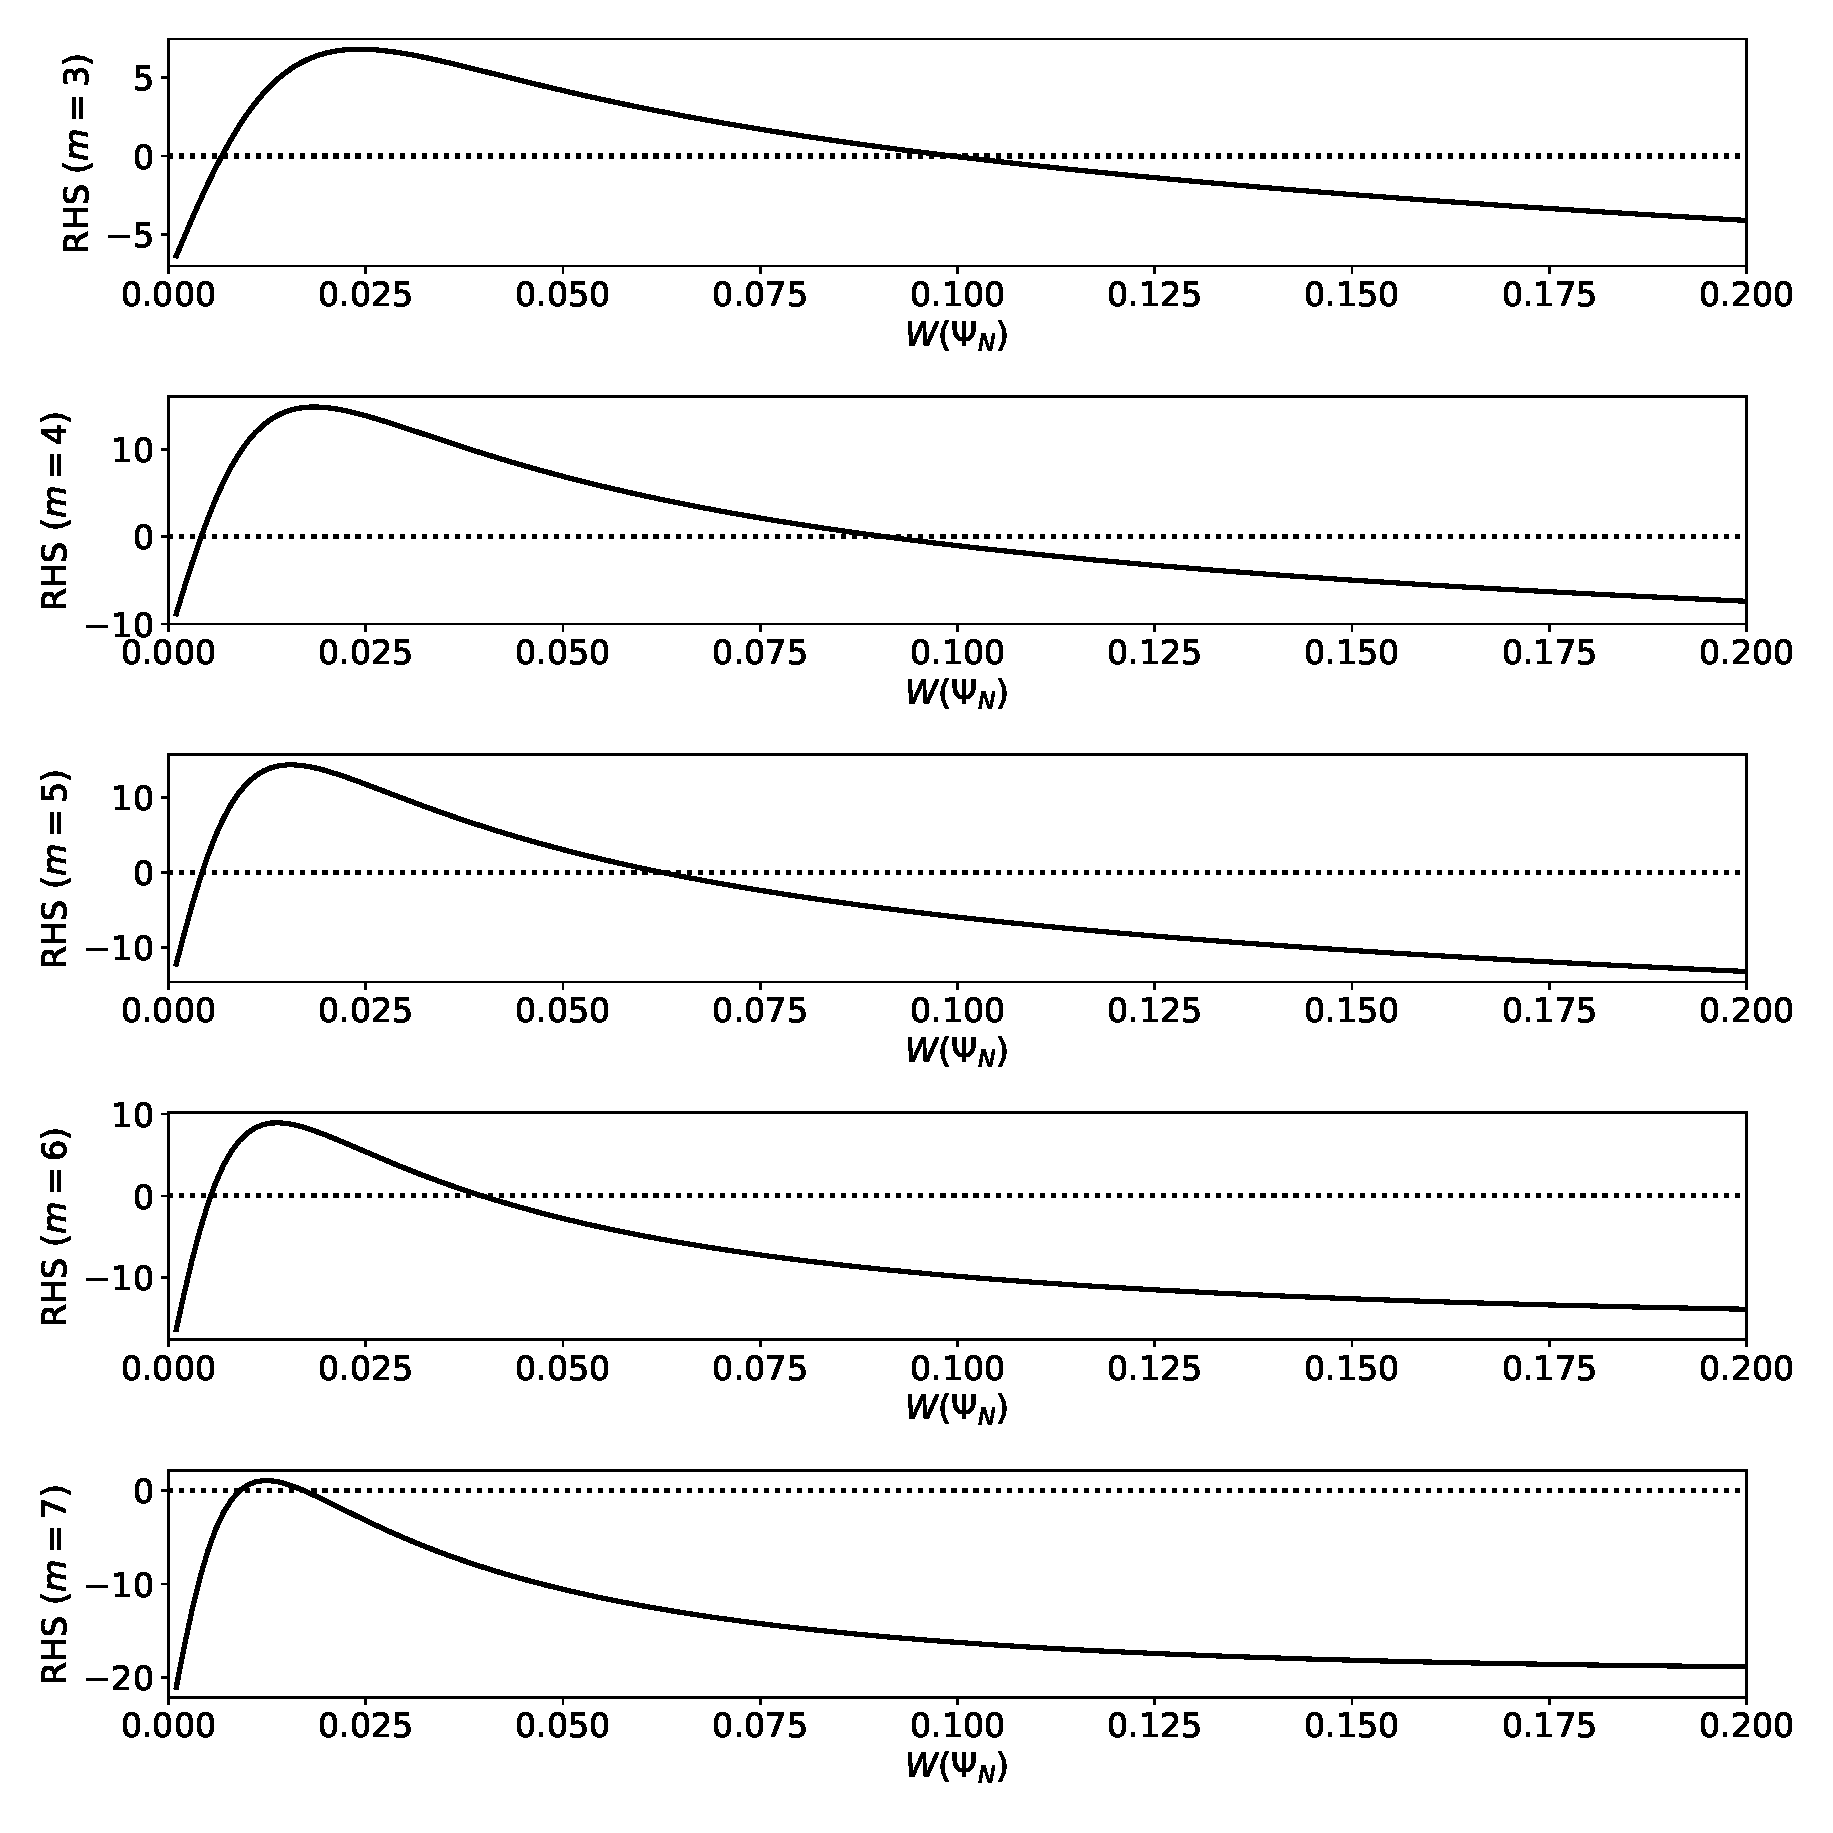
\includegraphics[height=6in]{Fig14.eps}}
\caption{Right-hand sides of modified Rutherford equations for $m=3/n=1$, $4/1$, $5/1$, $6/1$, and $7/1$ tearing modes in NSTX discharge 139057 at $t=557$\, ms.}\label{fig14}
\end{figure}

\begin{figure}
\centerline{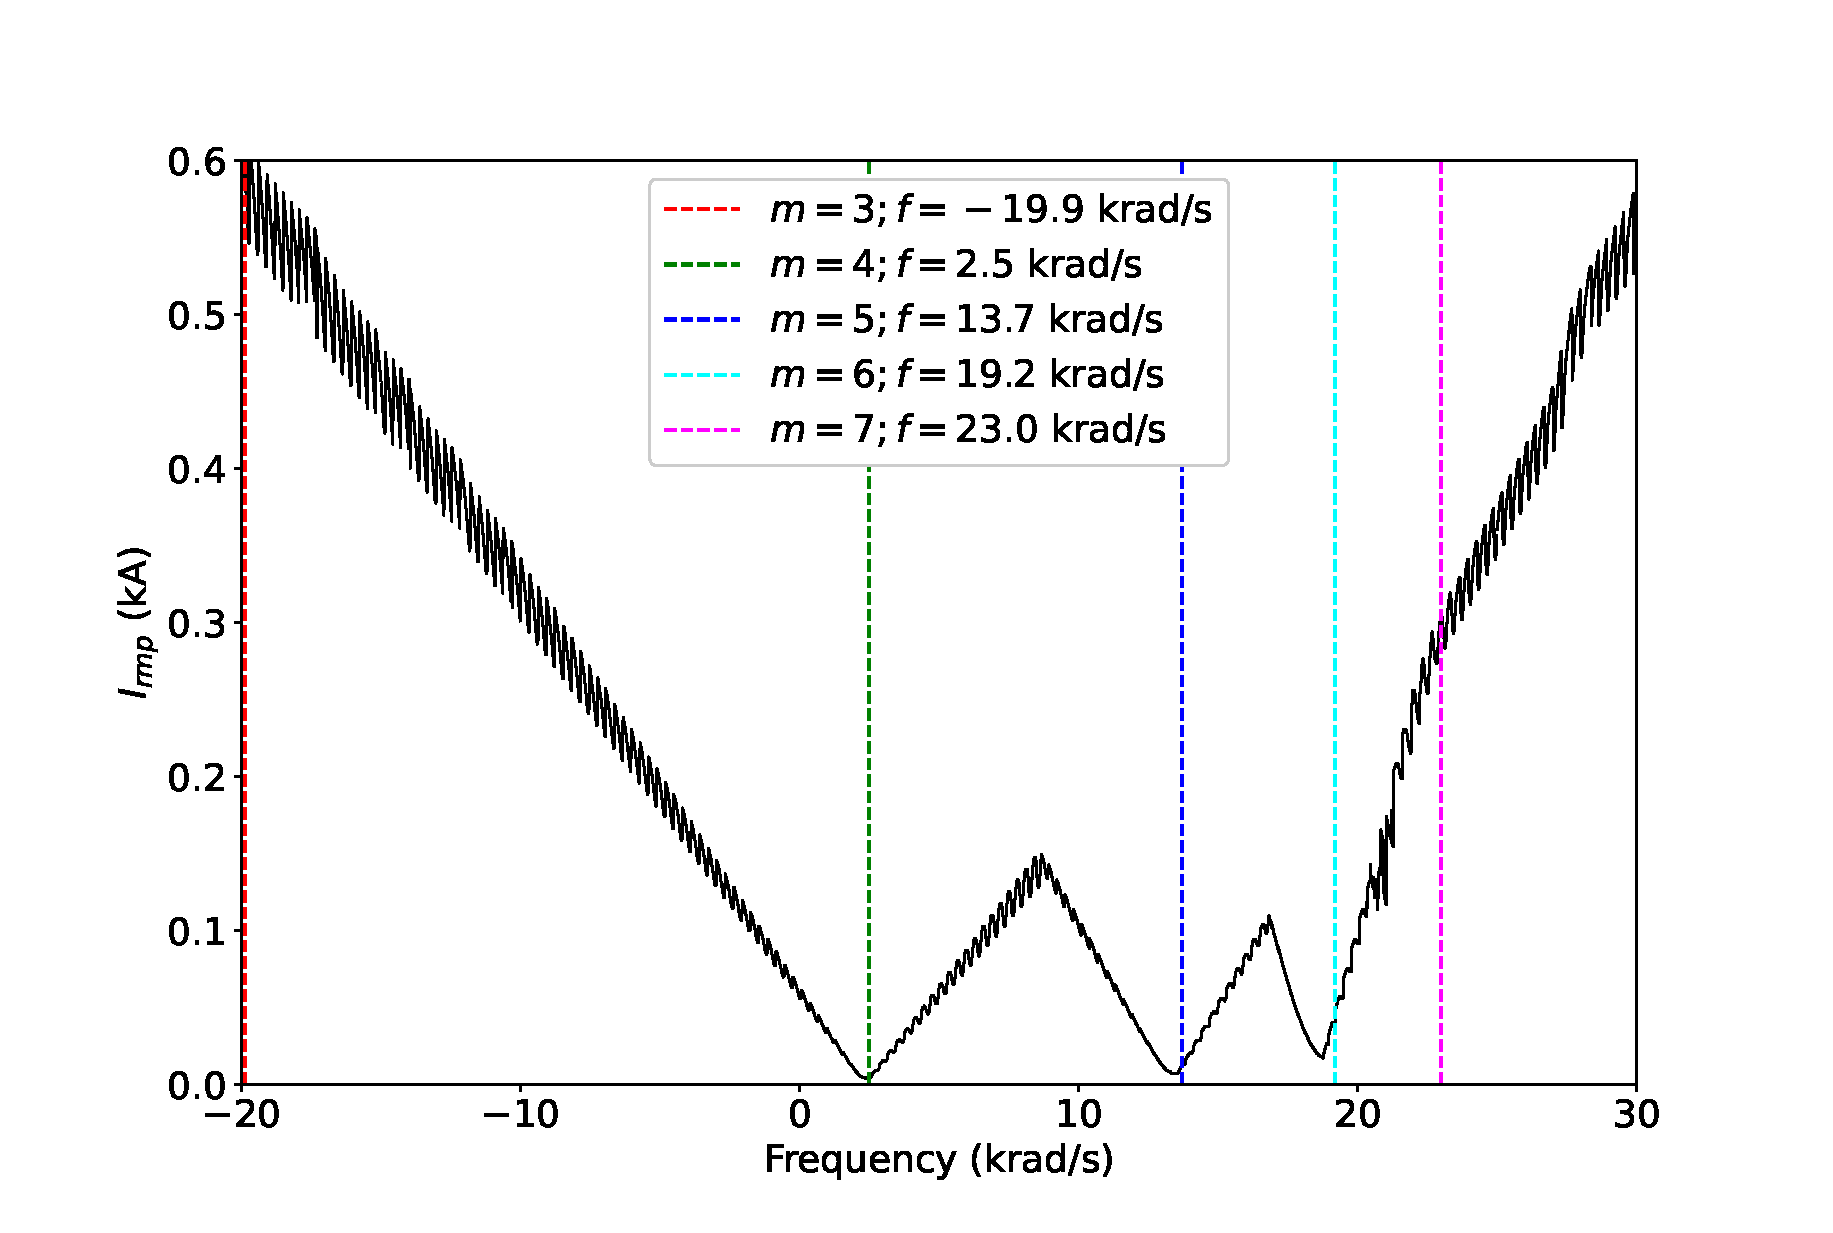
\includegraphics[height=5in]{Fig15.eps}}
\caption{Critical $n=1$ RMP coil current pulse amplitude required to trigger an $m=4/n=1$ NTM in NSTX discharge 139057 
as a function of the pulse frequency for a pulse duration of 20 ms.}\label{fig15}
\end{figure}

\end{document}